%!TEX program = xelatex
\documentclass{ctexbeamer}

\usepackage[bluetheme]{ustcbeamer}

                          %%% ustcbeamer说明 %%%%
%% 宏包使用了TikZ代码形式的背景文件(在子文件夹theme中),默认选项"bluetheme",是科大校徽的蓝色;此外ustcbeamer还内置了红色和黑色主题"redtheme","blacktheme"。

                        %%% 自定义你的主题颜色 %%%
%% 一旦使用了下述命令就会覆盖ustcbeamer的内置颜色选项,你可以设置自己喜欢的RGB色值:
% \definecolor{themecolor}{RGB}{0,150,0} % 这是绿色主题
% \definecolor{themecolor}{RGB}{0,150,150} % 青色主题,也蛮好看的

%% 注意小写rgb和大写RGB表示的色值相差255倍,即RGB{255,255,255}=rgb{1,1,1};
% \definecolor{themecolor}{rgb}{0,0.5,0.3} % 深绿色主题

%% 建议自定义的主题颜色选择偏深色
%%%%%%%%%%%%%%%%%%%%%%%%%%%%%%%%%%%%%%%%%%%%%%%%%%%%%%%%%%%%%%%%%%%%%%


\title[PrismNet]{
    Predicting dynamic cellular protein–RNA interactions by deep
learning using in vivo RNA structures
}
\author[Hong Jiang]{Reporter: Hong Jiang}
\institute[USTC]{
USTC,School of Life Sciences
}
\date{\today}
\begin{document}
%\section<⟨mode specification⟩>[⟨short section name⟩]{⟨section name⟩}
%小于等于六个标题为恰当的标题

%--------------------
%标题页
%--------------------
\maketitleframe
%--------------------
%目录页
%--------------------
%beamer 101
\begin{frame}%
  \frametitle{Outline}%
  \tableofcontents[hideallsubsections]%仅显示节
  %\tableofcontents%显示所节和子节
\end{frame}%
%--------------------
%节目录页
%--------------------
\AtBeginSection[]{
  \setbeamertemplate{footline}[footlineoff]%取消页脚
  \begin{frame}%
    \frametitle{Outline}
    %\tableofcontents[currentsection,subsectionstyle=show/hide/hide]%高亮当前节,不显示子节
    \tableofcontents[currentsection,subsectionstyle=show/show/hide]%show,shaded,hide
  \end{frame}
  \setbeamertemplate{footline}[footlineon]%添加页脚
}
%--------------------
%子节目录页
%--------------------
\AtBeginSubsection[]{
  \setbeamertemplate{footline}[footlineoff]%取消页脚
  \begin{frame}%
    \frametitle{Outline}
    %\tableofcontents[currentsection,subsectionstyle=show/hide/hide]%高亮当前节,不显示子节
    \tableofcontents[currentsection,subsectionstyle=show/shaded/hide]%show,shaded,hide
  \end{frame}
  \setbeamertemplate{footline}[footlineon]%添加页脚
}

\section{CNN}
\subsection{Introduction}
\begin{frame}
  \frametitle{PrismNet}
  \begin{figure}[H]
    \centering
    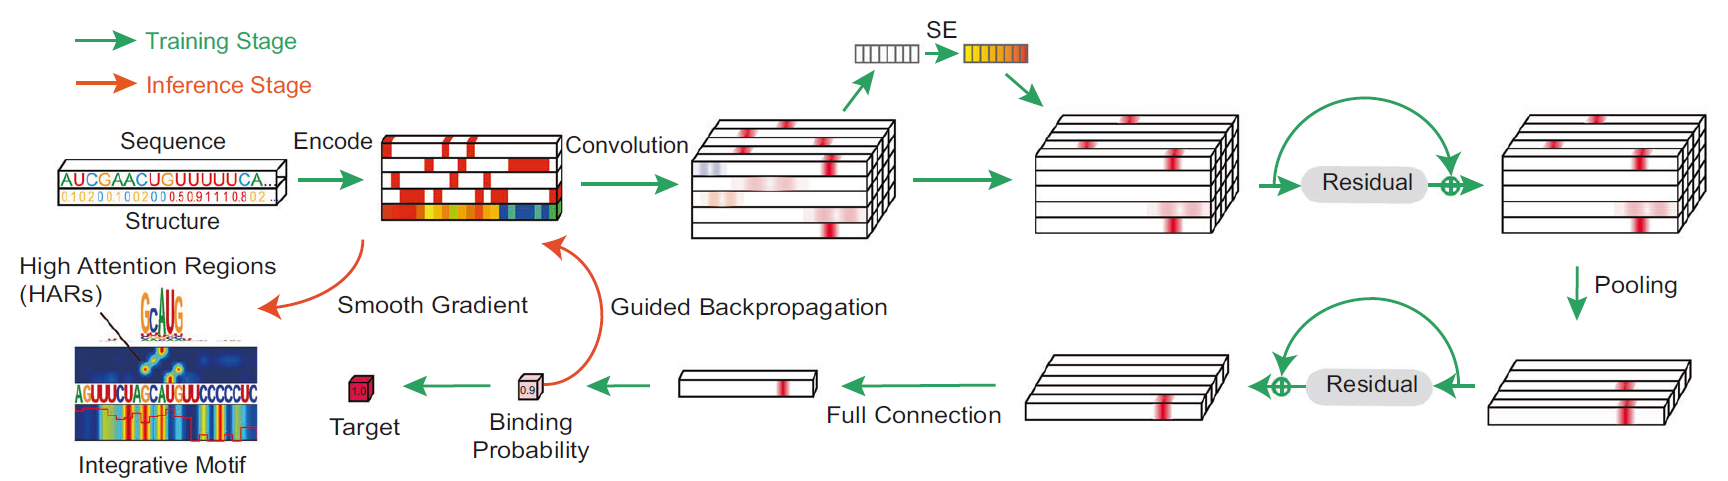
\includegraphics[width=0.95\textwidth]{./figures/CNN.png}
    \caption{PrismNet}
    \label{fig:cnn}
  \end{figure}
  \pause
  In this section, I will explain the terms in this network and it's input and output data structure.
\end{frame}

\begin{frame}
  \frametitle{Learning}
  \begin{columns}[T]
    \begin{column}{0.5\textwidth}
      \begin{itemize}
        \item Learn the Model Parameters and Hyperparameters; \\
        \item Make inferences about the world \\
      \end{itemize}
    \end{column}
    \begin{column}{0.5\textwidth}
      \begin{figure}[H]
        \raggedleft
        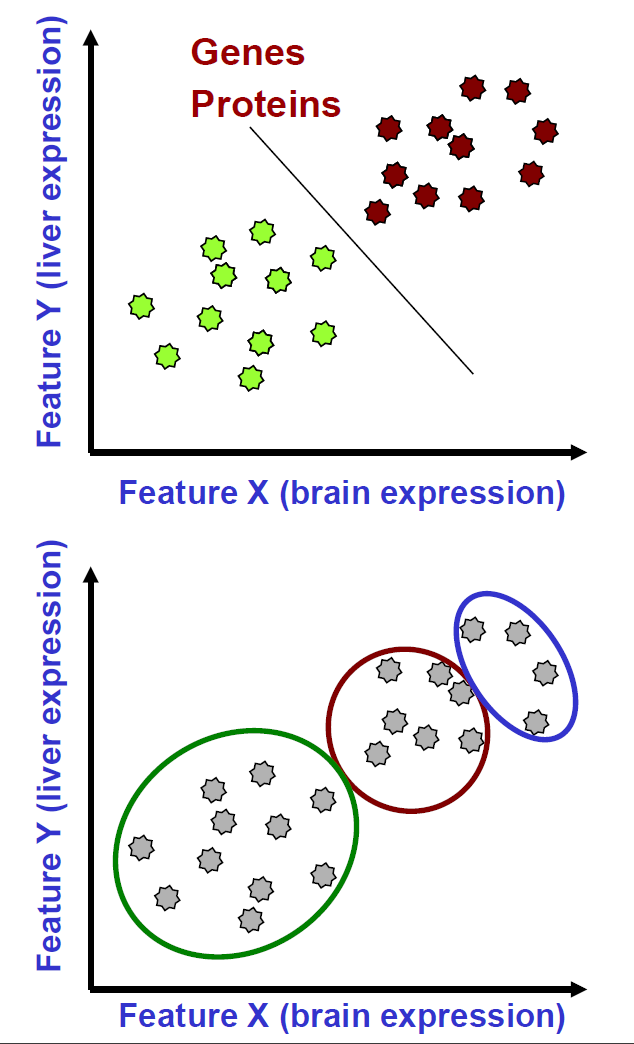
\includegraphics[width=0.7\textwidth]{./figures/learning.png}
        %\caption{Classification & Clustering}
        \label{fig:learning}
      \end{figure}
    \end{column}
  \end{columns}
\end{frame}

\subsection{Inspiration}
\begin{frame}
  \frametitle{Inspiration for Neural Network}
  \begin{figure}[H]
    \centering
    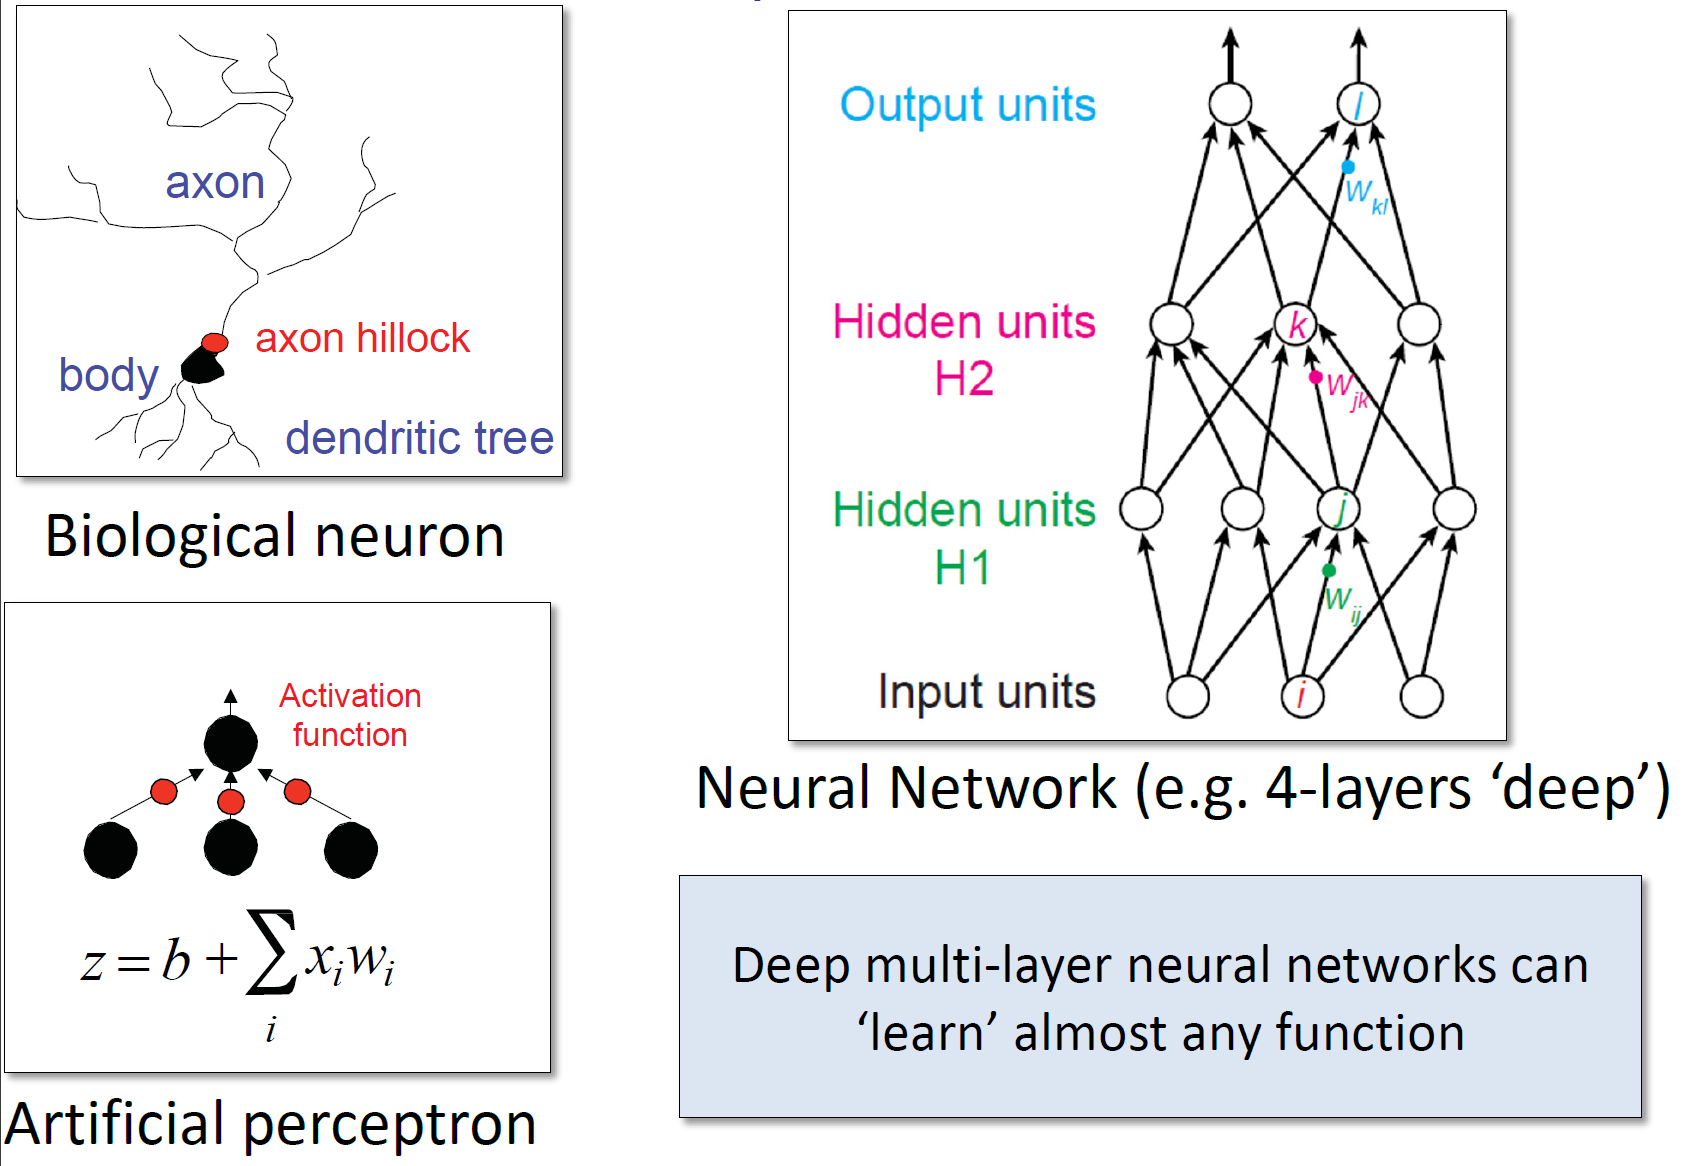
\includegraphics[width=0.8\textwidth]{./figures/NN.png}
    \caption{How the brain works inspired artificial “neural"networks}
    \label{fig:nn}
  \end{figure}
\end{frame}

\begin{frame}
  \frametitle{Motivation for CNN}
  \begin{figure}[H]
    %\centering
    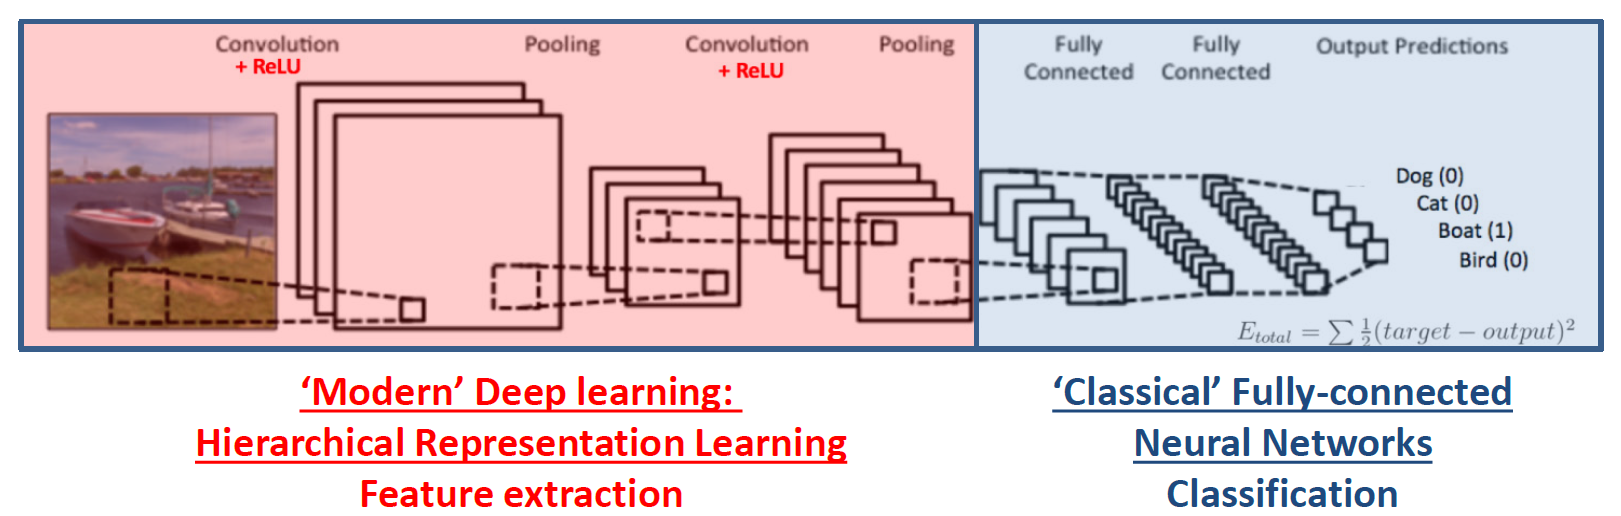
\includegraphics[width=0.95\textwidth]{./figures/motivation.png}
    %\caption{PrismNet}
    \label{fig:motivation}
  \end{figure}
  \begin{figure}[H]
    %\centering
    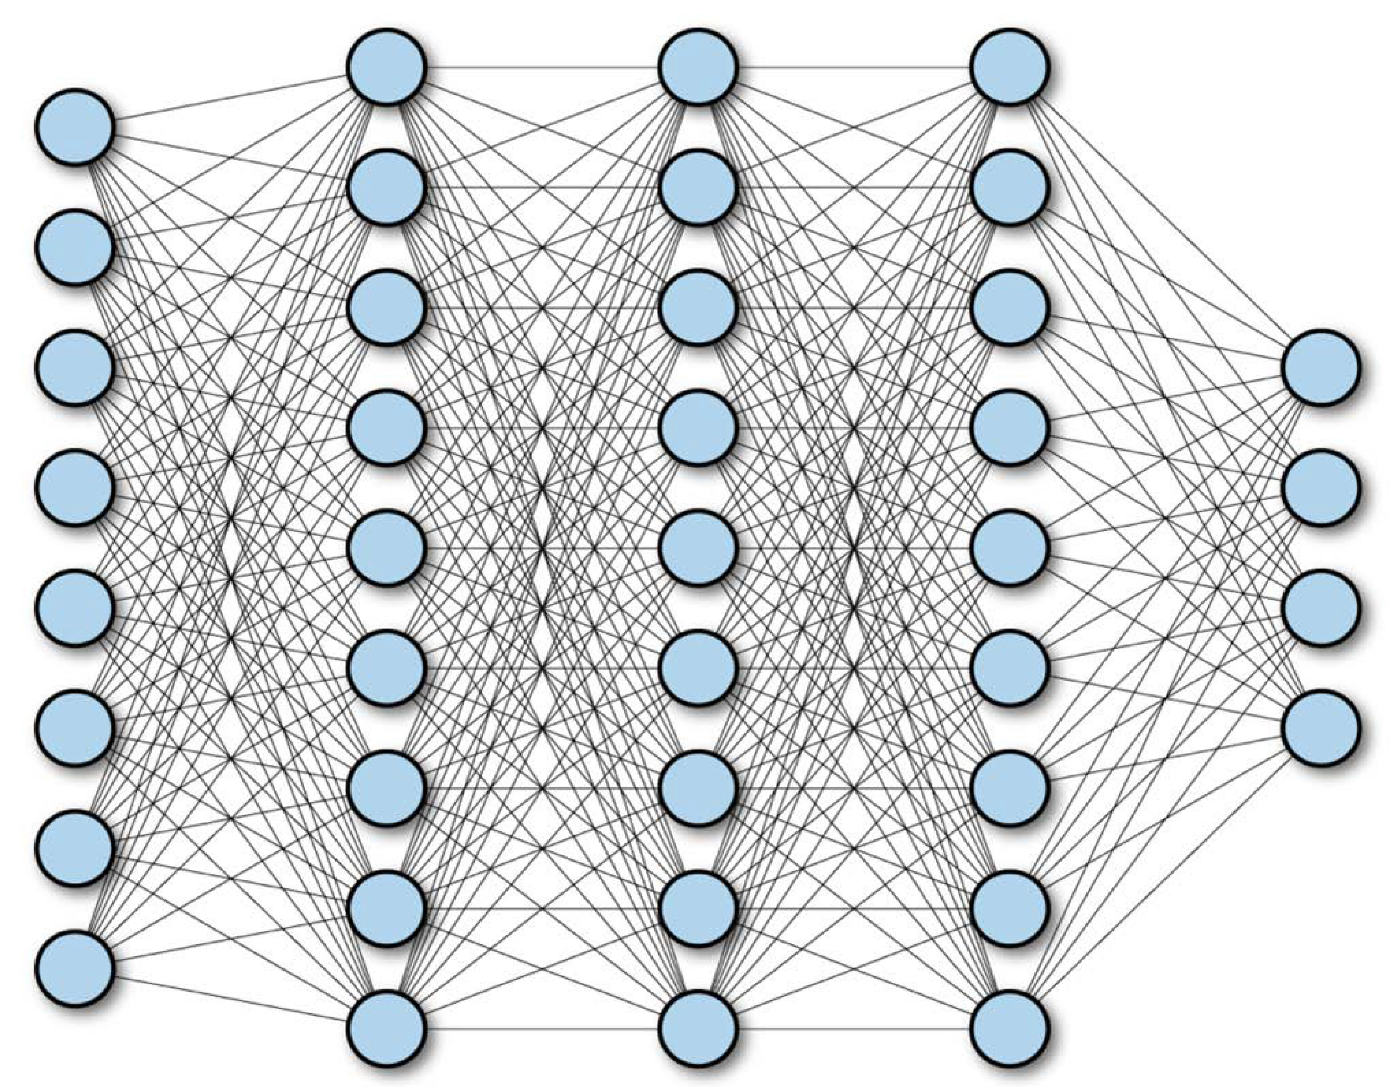
\includegraphics[width=0.3\textwidth]{./figures/fc_nn.png}
    \label{fig:fc_cnn}
  \end{figure}
\end{frame}

\subsection{Terms}
\begin{frame}
  \frametitle{Inspiration for CNN}
  \begin{figure}[H]
    \centering
    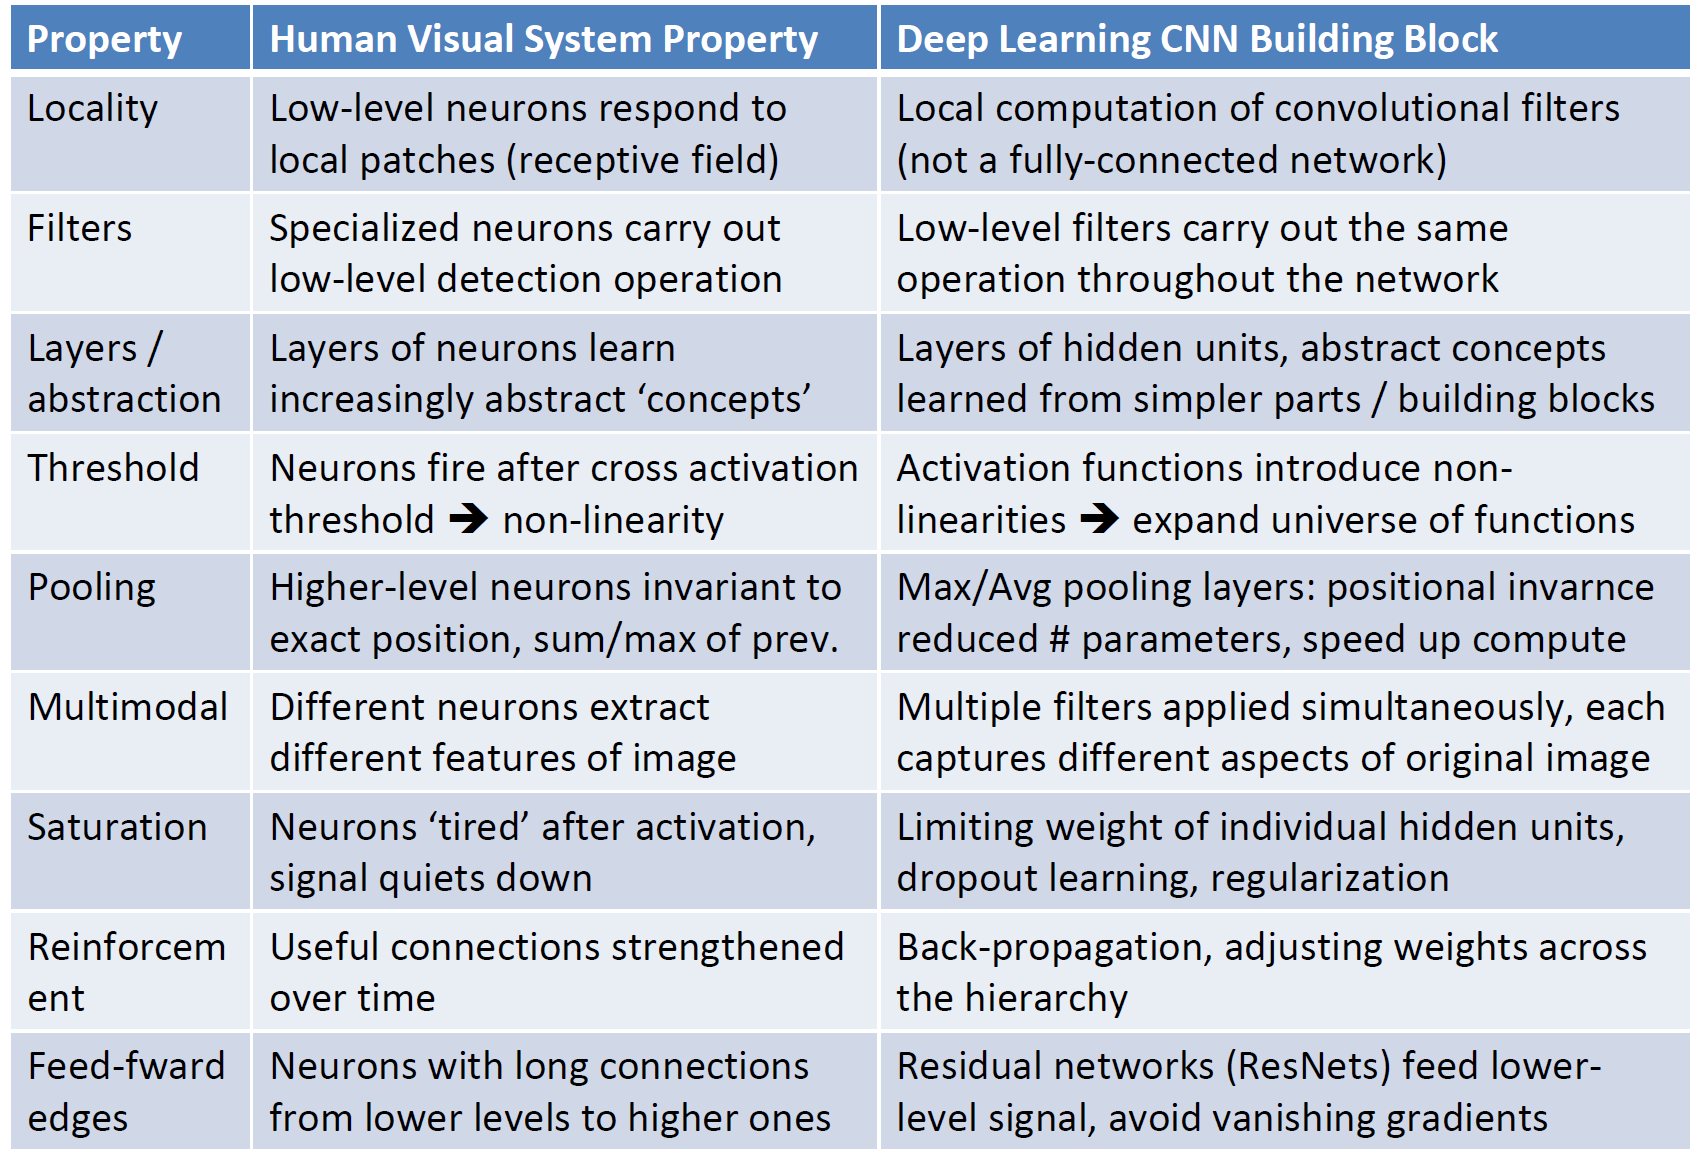
\includegraphics[width=0.95\textwidth]{./figures/cnn_brain.png}
    %\caption{How the brain works inspired artificial “neural"networks}
  \end{figure}
\end{frame}

\begin{frame}
  \frametitle{Convolution}
  \begin{figure}[H]
    \centering
    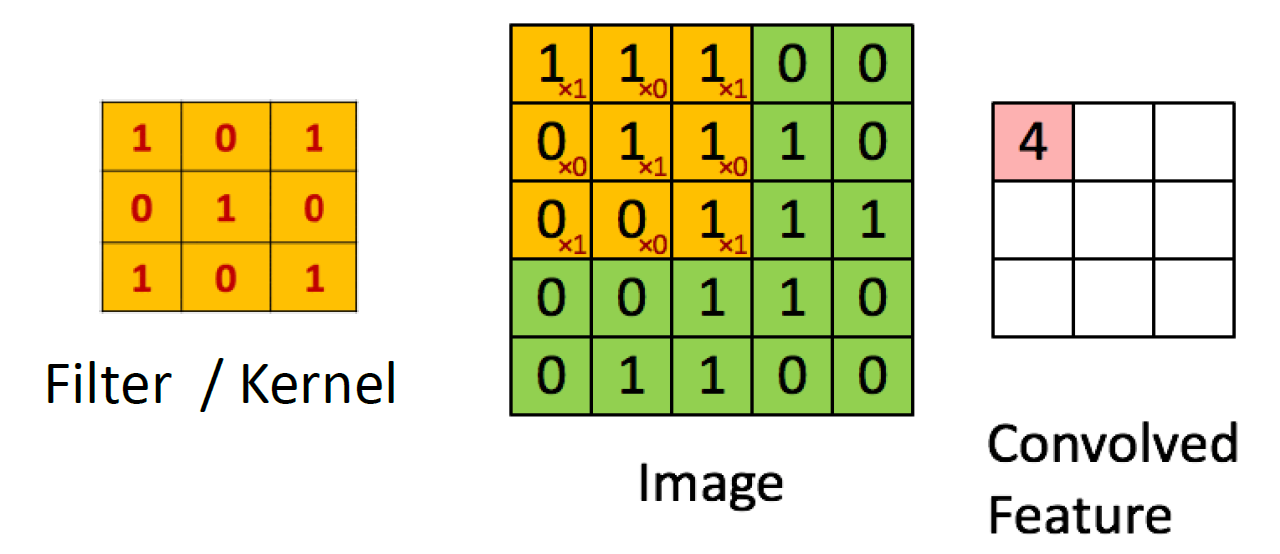
\includegraphics[width=0.5\textwidth]{./figures/convolution.png}
    %\caption{Convolution}
    \label{fig:convolution}
  \end{figure}
  \begin{block}{Padding}
    \begin{itemize}
      \item Same convolution: zero pad input so output is same size as input dimensions
      \item Valid-only convolution: output only when entire kernel contained in input (shrinks output)
      \item Full convolution: zero pad input so output is produced whenever an output value contains at least one input value (expands output)
    \end{itemize}
  \end{block}
  %SE: Apply after every convolution operation
  %avg_pool $+$ Linear $+$ ReLU $+$ Linear $+$ Sigmoid
\end{frame}

\begin{frame}
  \frametitle{Pooling}
  \begin{figure}[H]
    \centering
    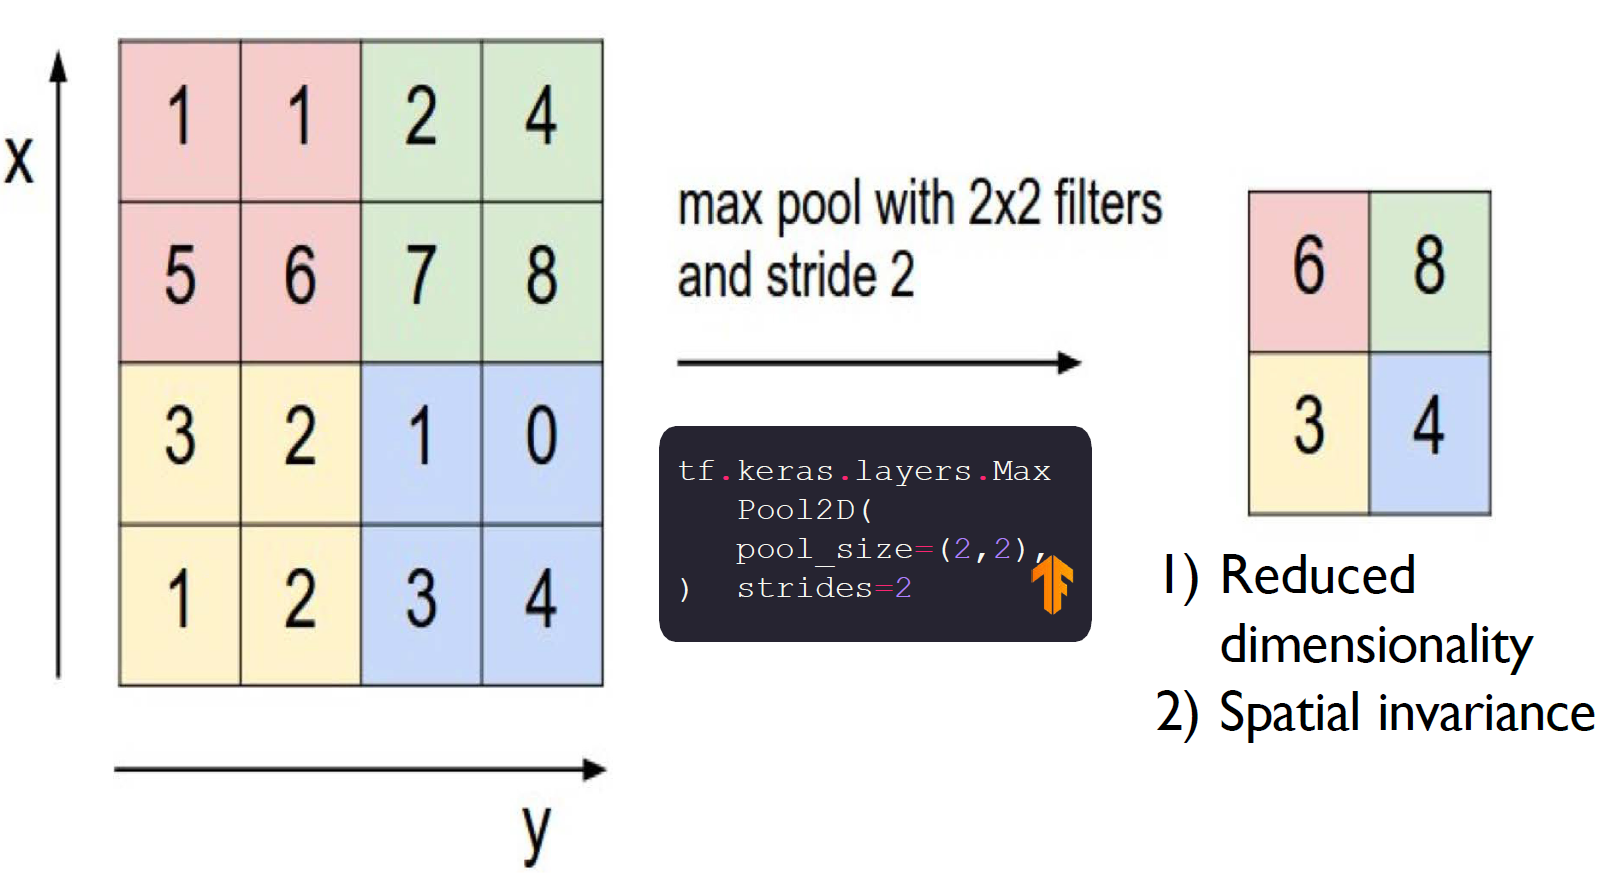
\includegraphics[width=0.6\textwidth]{./figures/pooling.png}
    %\caption{Polling}
    \label{fig:pooling}
  \end{figure}
  \begin{block}{Why Pooling}
    \begin{itemize}
      \item Positional Invariance (Detected Featues more Robust)
      \item Speed up Computation
    \end{itemize}
  \end{block}
  %SE: Apply after every convolution operation
  %avg_pool $+$ Linear $+$ ReLU $+$ Linear $+$ Sigmoid
\end{frame}

\begin{frame}
  \frametitle{Non Linearity}
  \begin{columns}[T]
    \begin{column}{0.5\textwidth}
      \begin{figure}[H]
        \raggedright
        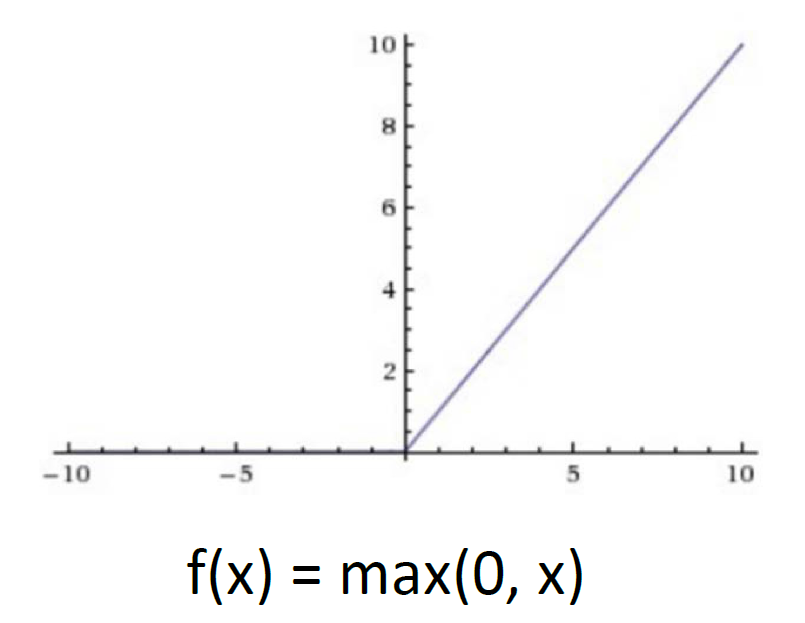
\includegraphics[width=\textwidth]{./figures/ReLu.png}
        \caption{REctified Linear Unit}
        \label{fig:relu}
      \end{figure}
    \end{column}
    \begin{column}{0.5\textwidth}
      \begin{figure}[H]
        \raggedleft
        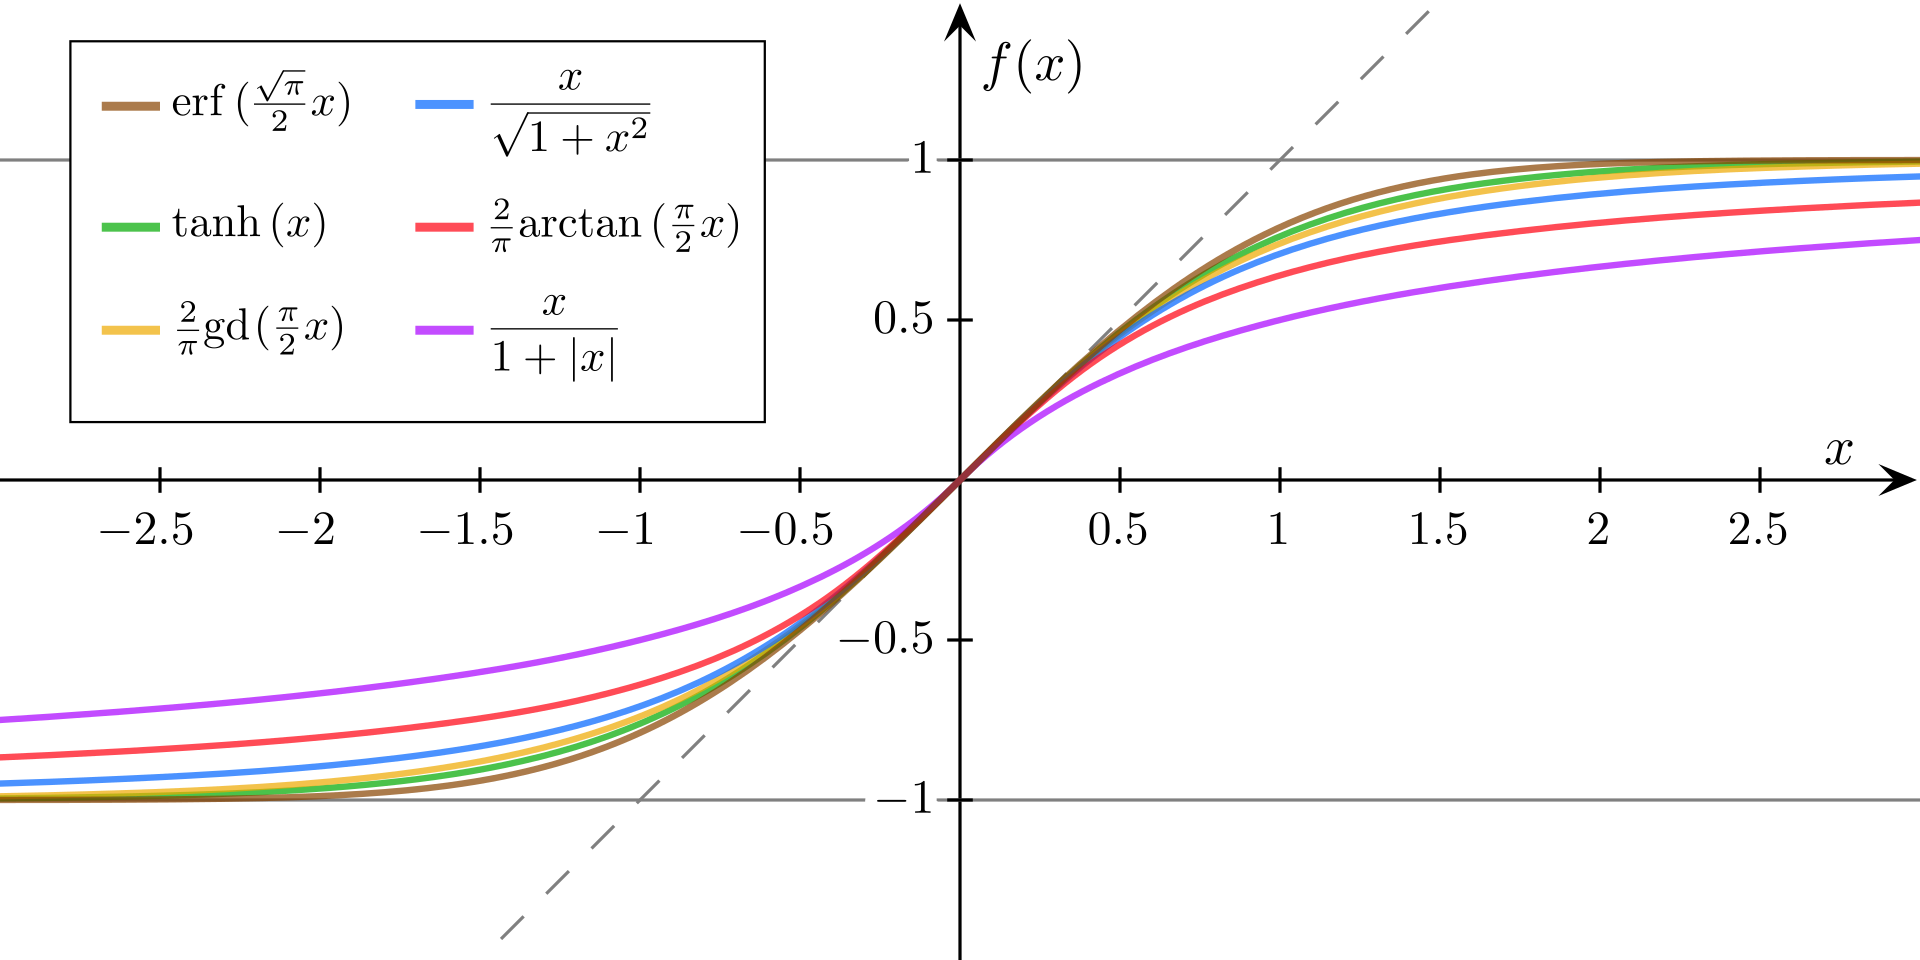
\includegraphics[width=\textwidth]{./figures/sigmoid.png}
        \caption{Sigmoid Function}
        \label{fig:sigmoid}
      \end{figure}
    \end{column}
  \end{columns}
\end{frame}

\begin{frame}
  \frametitle{Back Propagation}
  \begin{figure}[H]
    \centering
    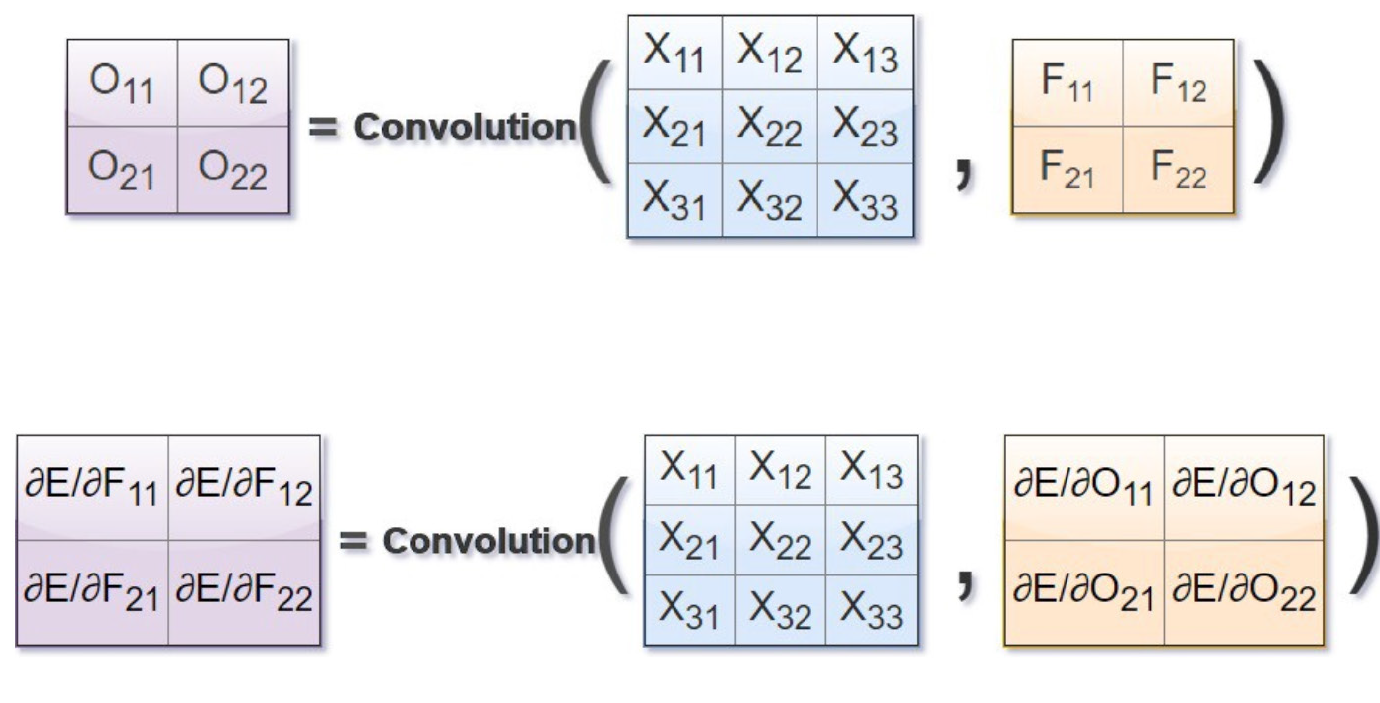
\includegraphics[width=\textwidth]{./figures/bp.png}
    \caption{Backpropagation of convolution}
    \label{fig:bp}
  \end{figure}
  %SE: Apply after every convolution operation
  %avg_pool $+$ Linear $+$ ReLU $+$ Linear $+$ Sigmoid
\end{frame}

\begin{frame}
  \frametitle{Trainig and Inference}
  \begin{columns}[T]
    \begin{column}{0.5\textwidth}
      \begin{figure}[H]
        \raggedright
        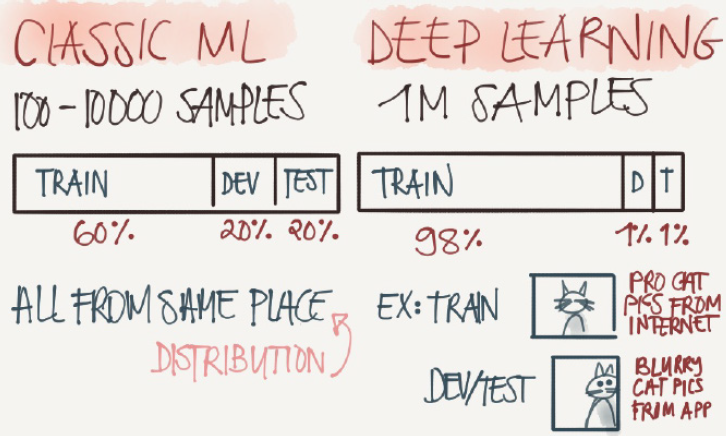
\includegraphics[width=\textwidth]{./figures/training.png}
        \caption{Training, Validation and Testing}
        \label{fig:training}
      \end{figure}
    \end{column}
    \begin{column}{0.5\textwidth}
      \begin{figure}[H]
        \raggedleft
        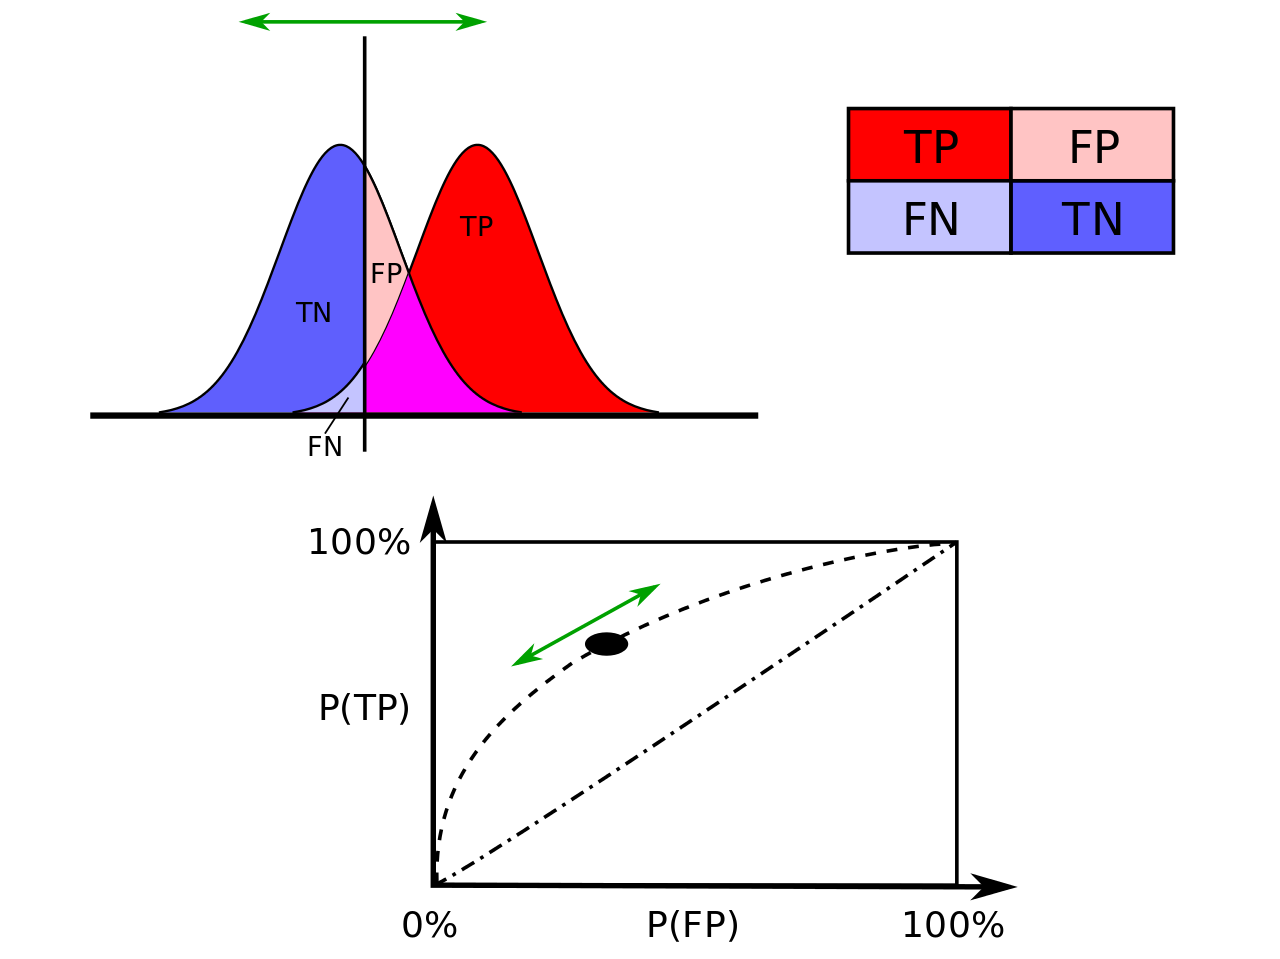
\includegraphics[width=\textwidth]{./figures/auc.png}
        \caption{Metrics for Performance}
        \label{fig:performance}
      \end{figure}
    \end{column}
  \end{columns}
\end{frame}

\begin{frame}
  \frametitle{PrismNet}
  \begin{figure}[H]
    \centering
    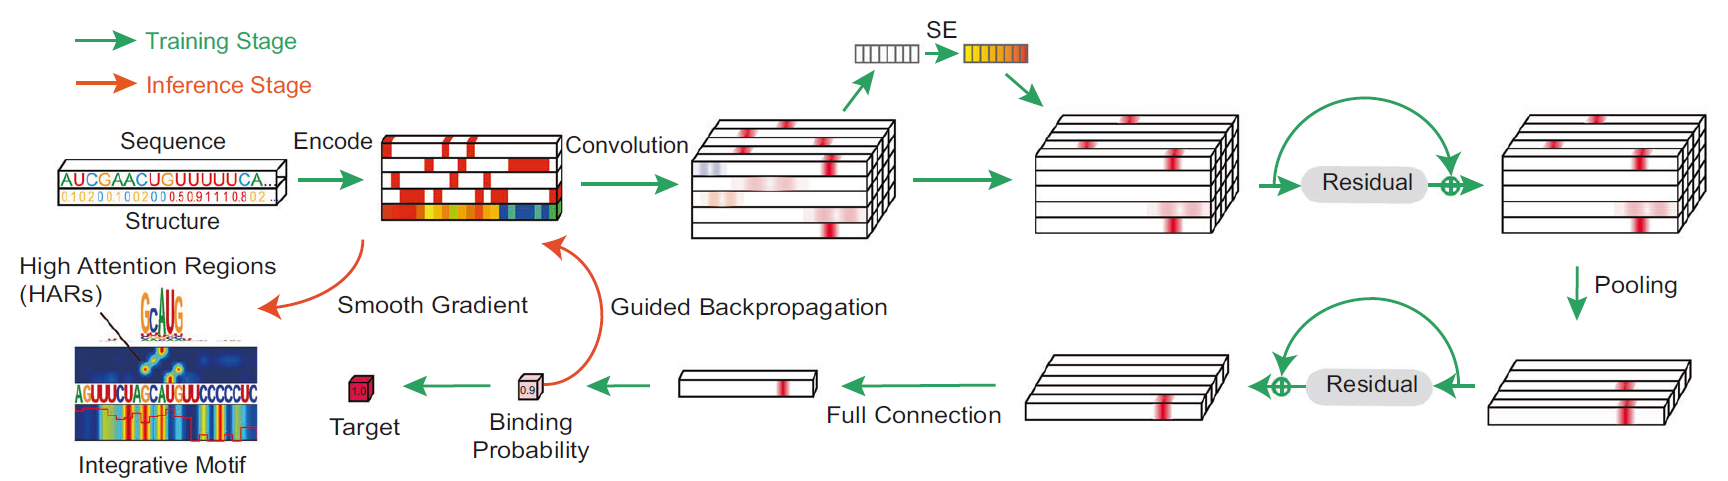
\includegraphics[width=\textwidth]{./figures/CNN.png}
    \caption{PrismNet}
    \label{fig:cnn}
  \end{figure}
  \begin{block}{SE}
    \begin{itemize}
      \item Apply after every convolution operation
      \item $Avg_pool$, $Linear$, $ReLU$, $Linear$, $Sigmoid$
    \end{itemize}
  \end{block}
\end{frame}

\section{Input and Output Data}
\subsection{Input Data}
\begin{frame}
  \frametitle{Encode Input Data}
  \begin{figure}[H]
    \raggedright
    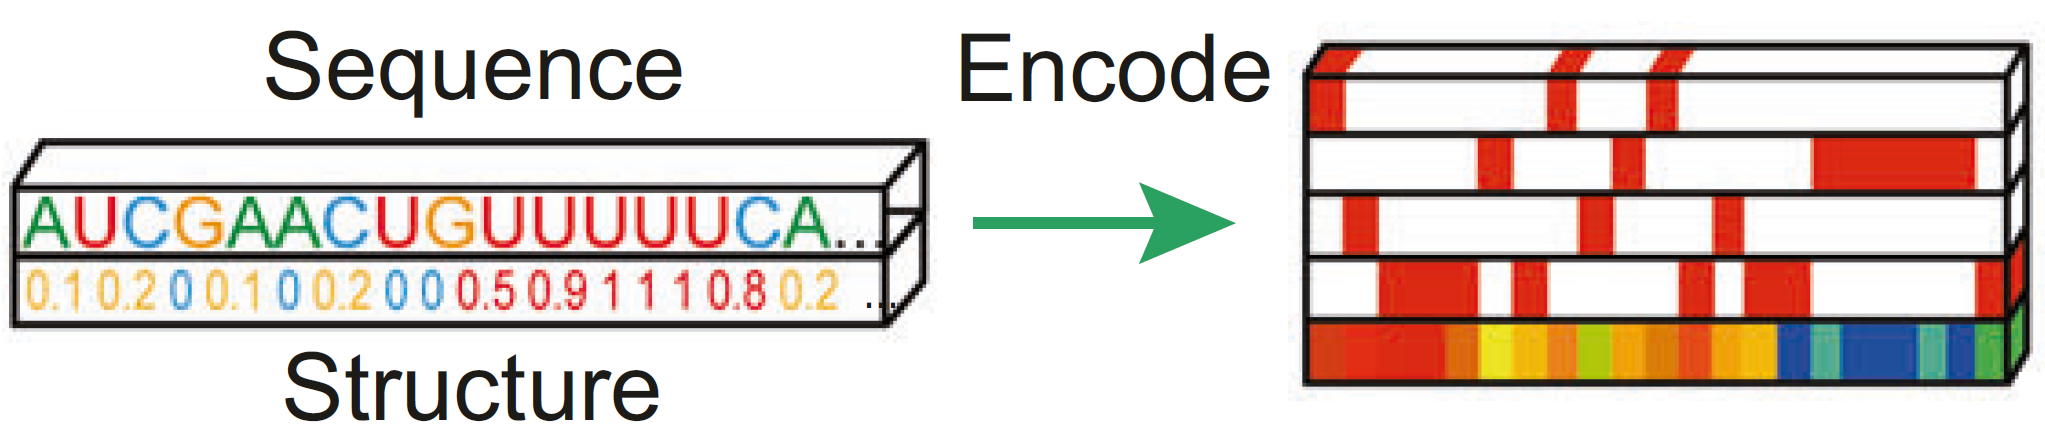
\includegraphics[width=0.85\textwidth]{./figures/input.png}
    %\caption{REctified Linear Unit}
    \label{fig:input}
  \end{figure}
  \begin{figure}[H]
    \raggedleft
    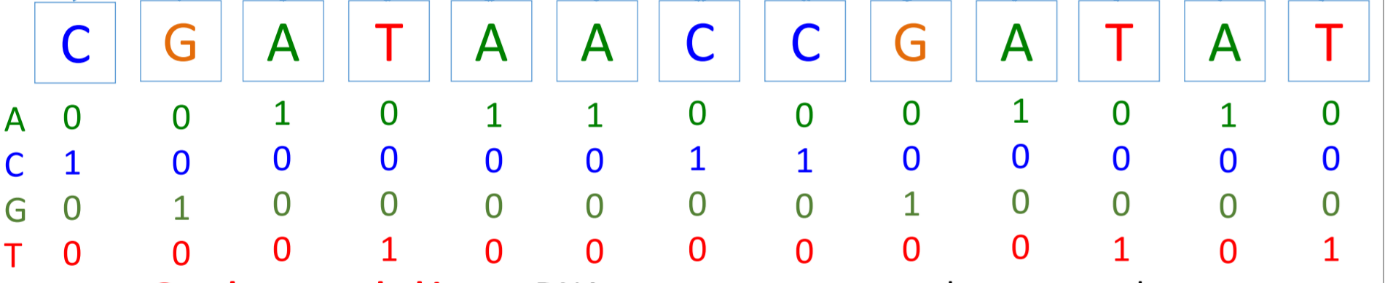
\includegraphics[width=0.85\textwidth]{./figures/onehot.png}
    %\caption{Sigmoid Function}
    \label{fig:onehot}
  \end{figure}
  \begin{block}{Description}
    The icSHAPE structure scores of each nucleotide of the CLIP experiment were encoded as a one-dimensional vector, together with the four-dimensional one-hot-encoded
    sequence as input
  \end{block}
\end{frame}

\begin{frame}
  \frametitle{icSHAPE structure scores}
  \begin{figure}[H]
    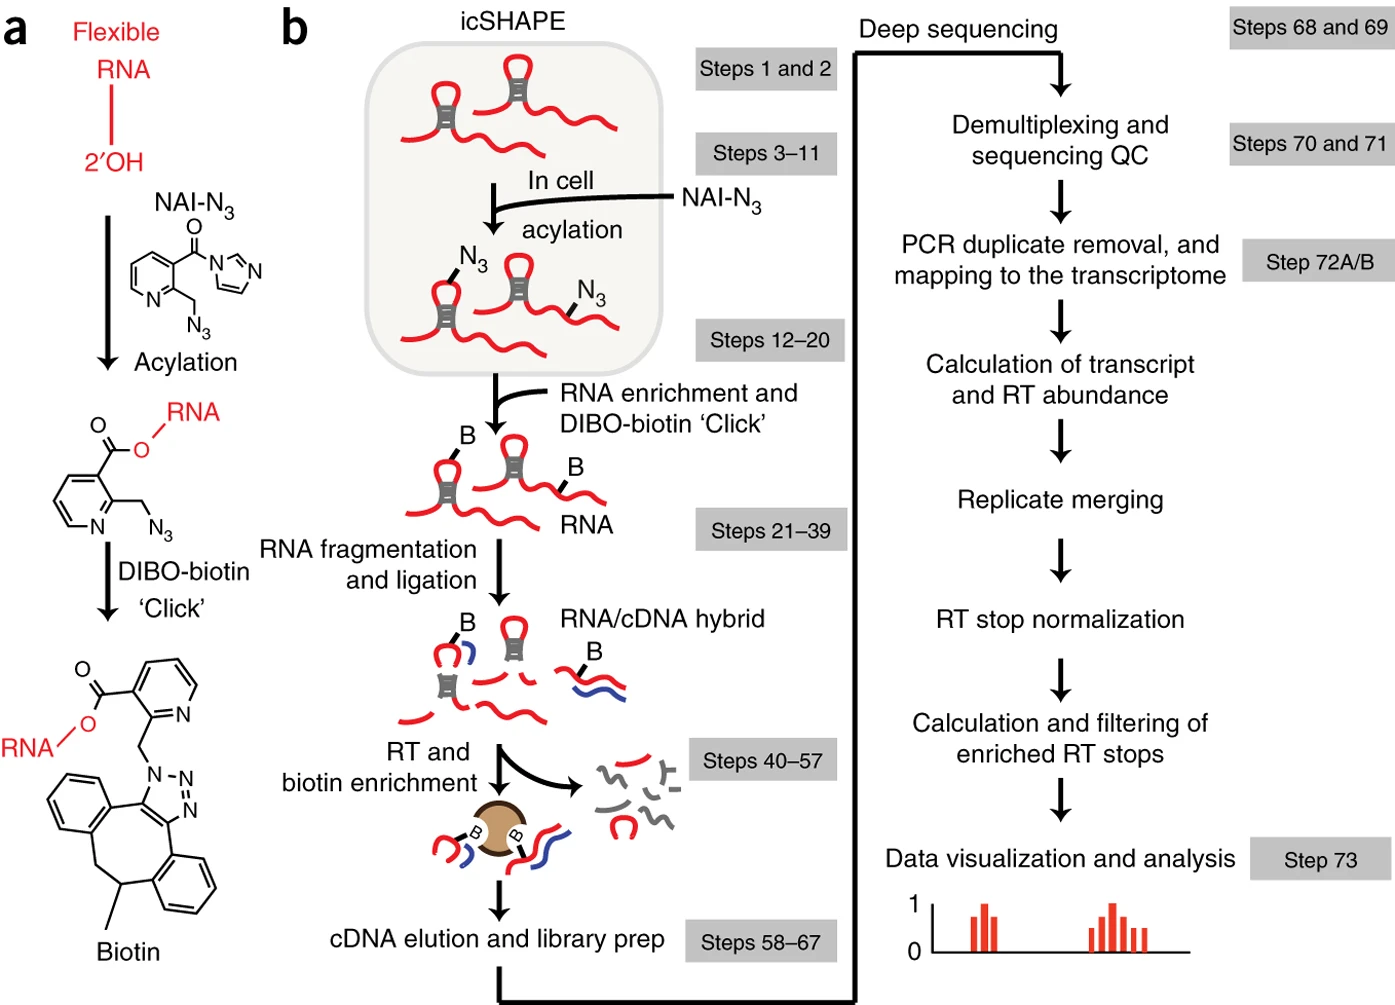
\includegraphics[width=0.75\textwidth]{./figures/shape.png}
    %\caption{REctified Linear Unit}
    \label{fig:icshape}
  \end{figure}
    \begin{figure}[H]
    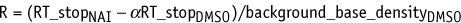
\includegraphics[width=0.75\textwidth]{./figures/score.png}
    %\caption{REctified Linear Unit}
    \label{fig:score}
  \end{figure}
\end{frame}

\subsection{Output Data}
\begin{frame}
  \frametitle{Clip Experiments}
  \begin{figure}[H]
    \center
    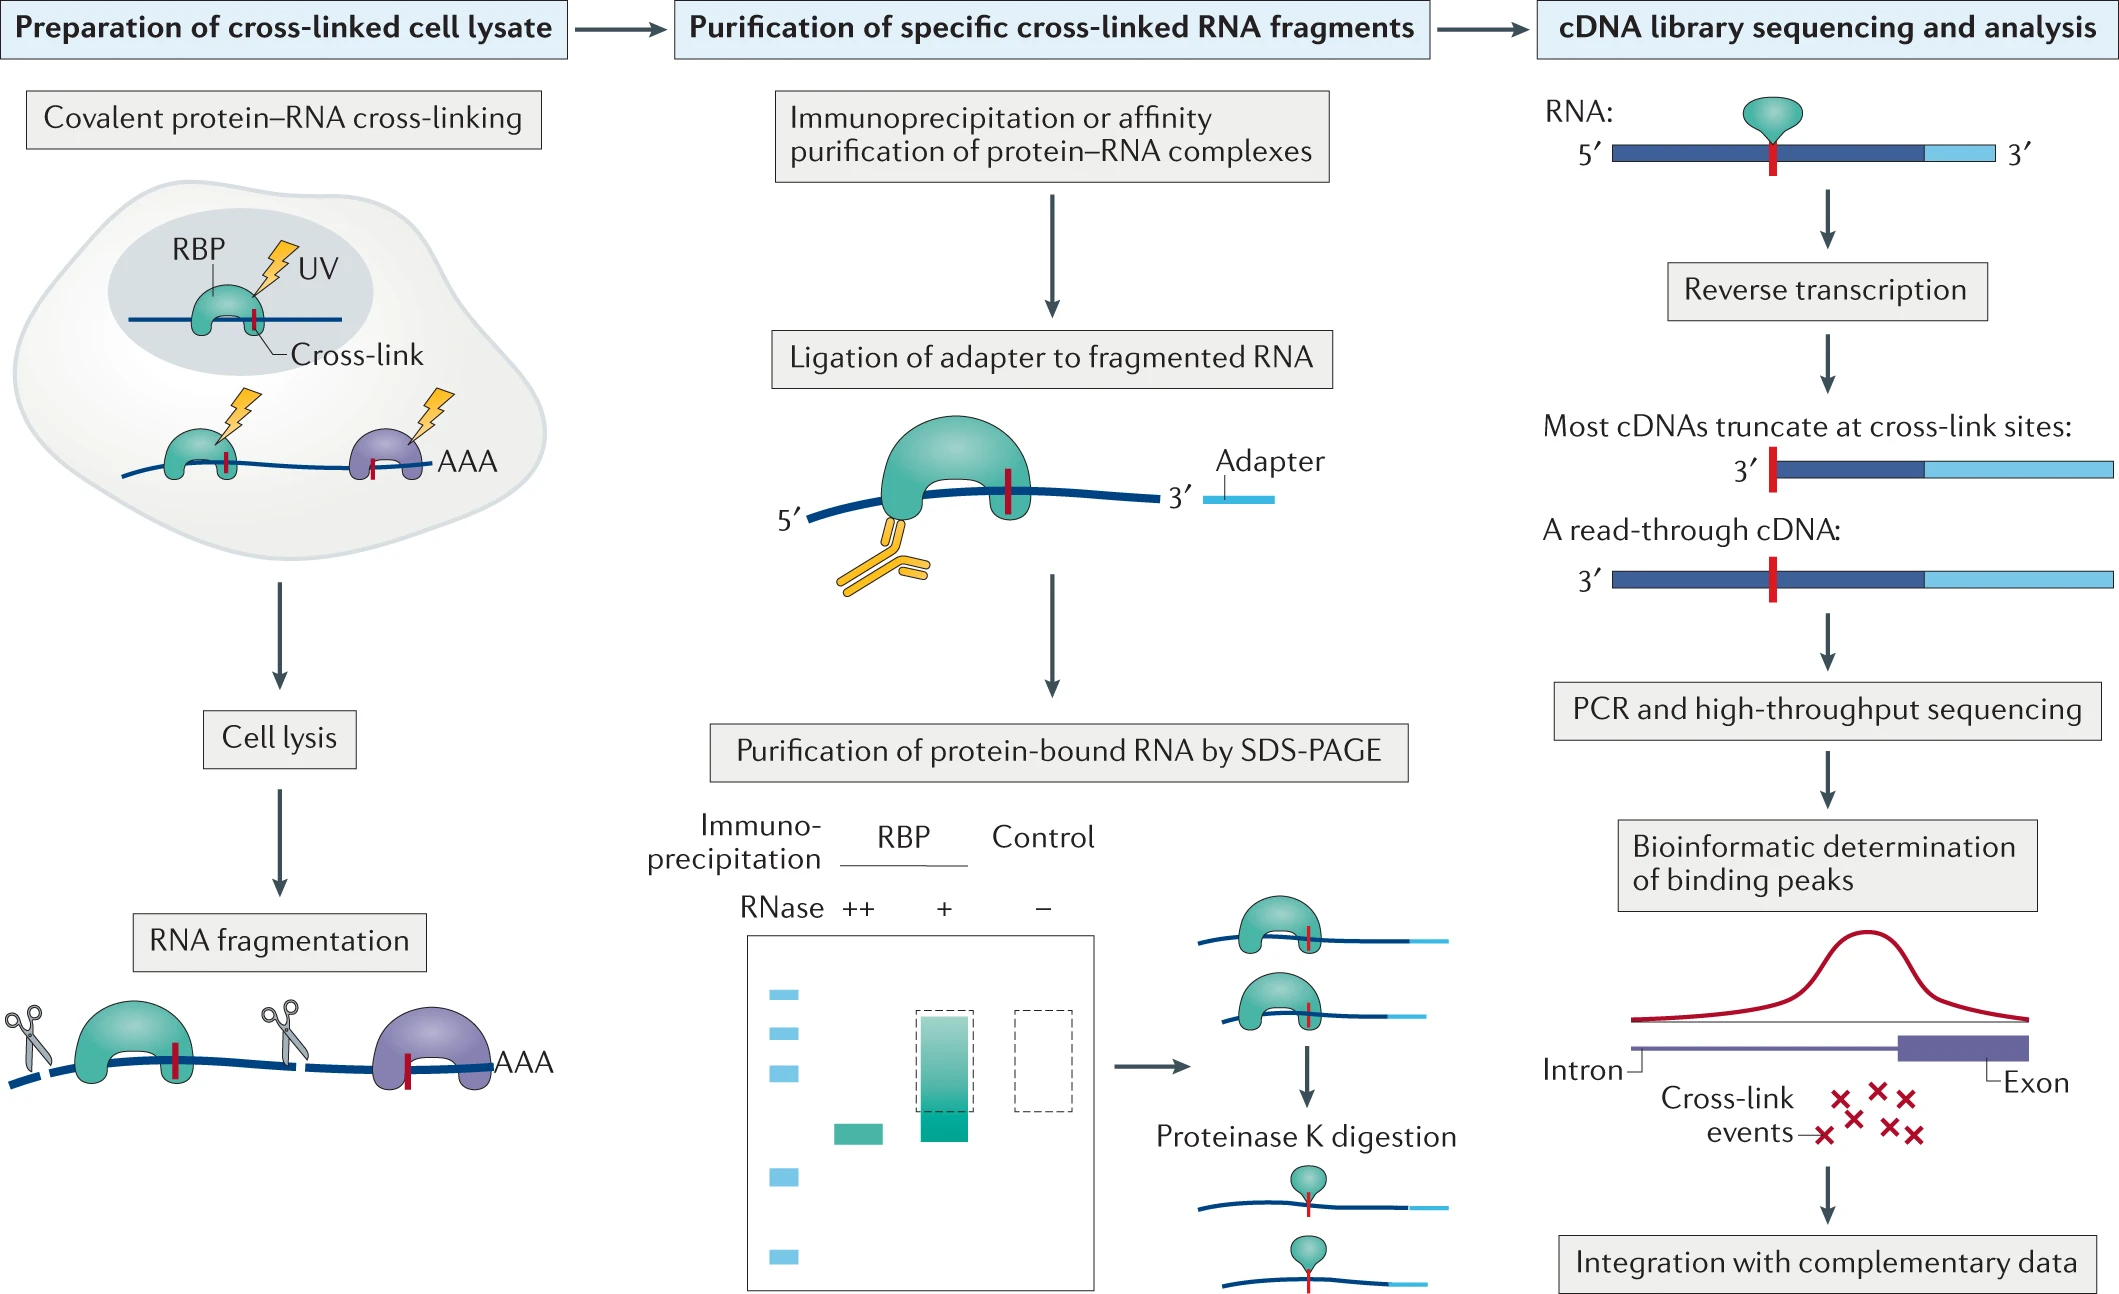
\includegraphics[width=0.85\textwidth]{./figures/clip.png}
    %\caption{REctified Linear Unit}
    \label{fig:clip}
  \end{figure}
  \begin{block}{Label}
  \begin{itemize}
    \item Training: 0/1
    \item Testing: The probability of being a reliable binding site
  \end{itemize} 
  \end{block}
\end{frame}

\section{Data Overview}

\begin{frame}
  \frametitle{$\Delta$ Structures and $\Delta$ RBP}
  \begin{columns}[T]
    \begin{column}{0.5\textwidth}
      \begin{figure}[H]
        \raggedright
        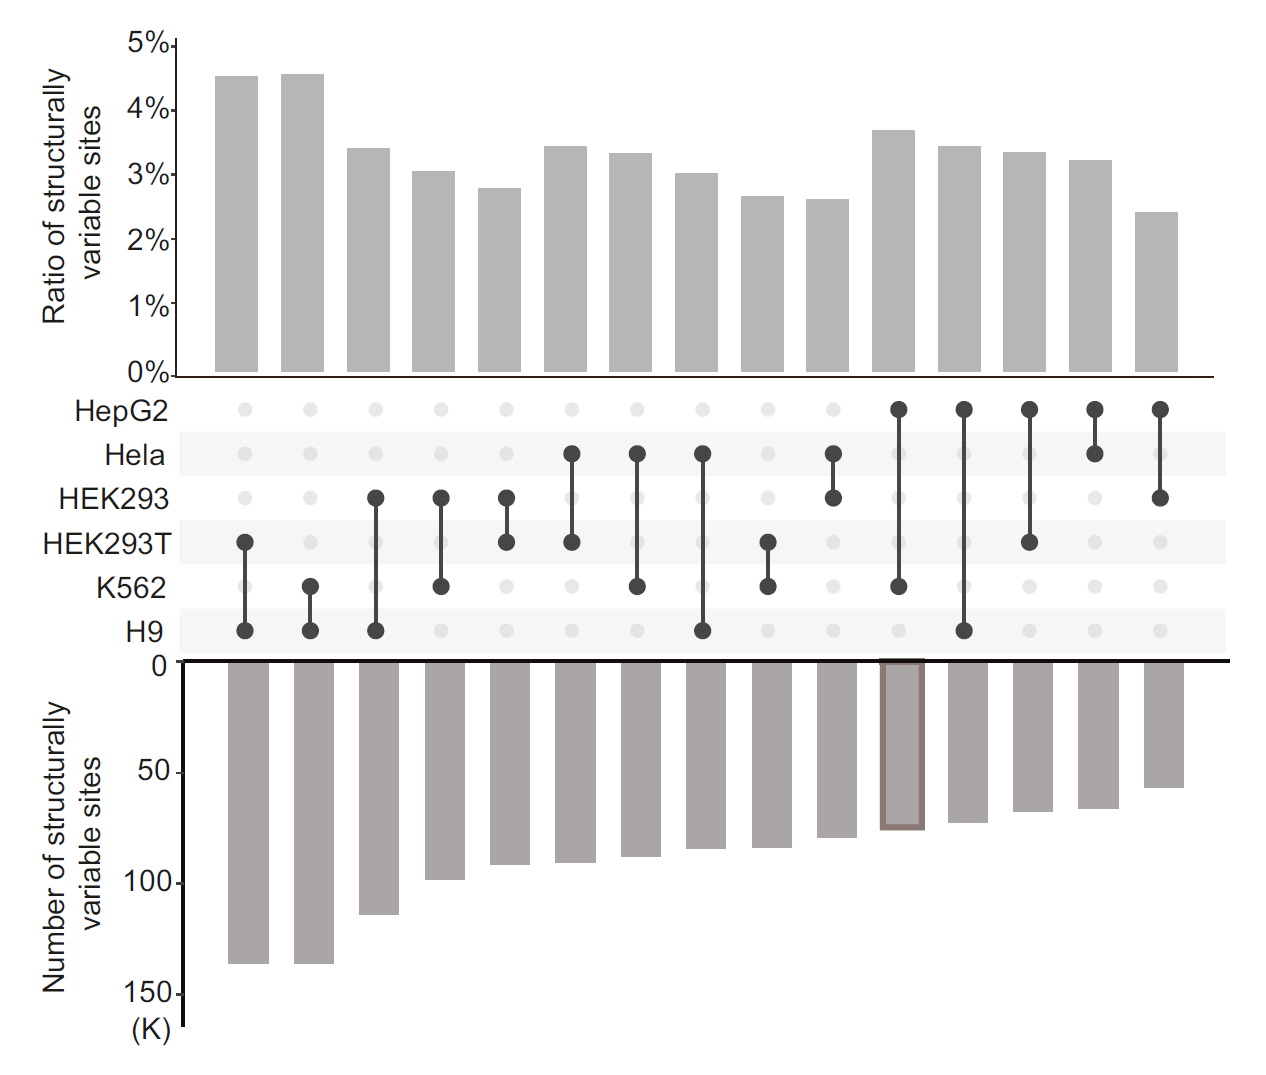
\includegraphics[width=\textwidth]{./figures/SV.png}
        \caption{most of the RNA structures are stable across all cell lines tested}
        \label{fig:sv}
      \end{figure}
    \end{column}
    \begin{column}{0.5\textwidth}
        \begin{figure}[H]
        \raggedleft
        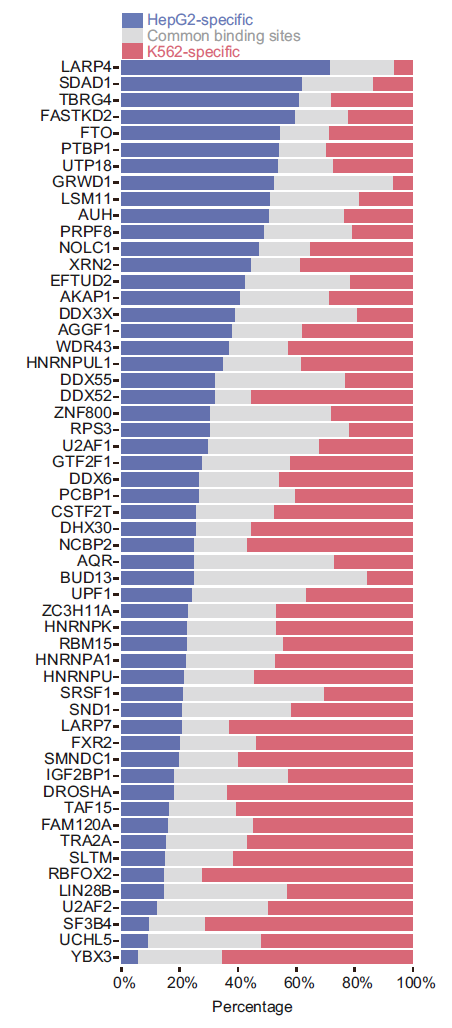
\includegraphics[width=0.5\textwidth]{./figures/binding_site.png}
        \caption{very different binding profiles for the same RBPs in
different cell lines}
        \label{fig:bs}
      \end{figure}
    \end{column}
  \end{columns}
\end{frame}

\begin{frame}
  \frametitle{Relation between Input and Output}
    \begin{columns}[T]
    \begin{column}{0.5\textwidth}
      \begin{figure}[H]
        \raggedright
        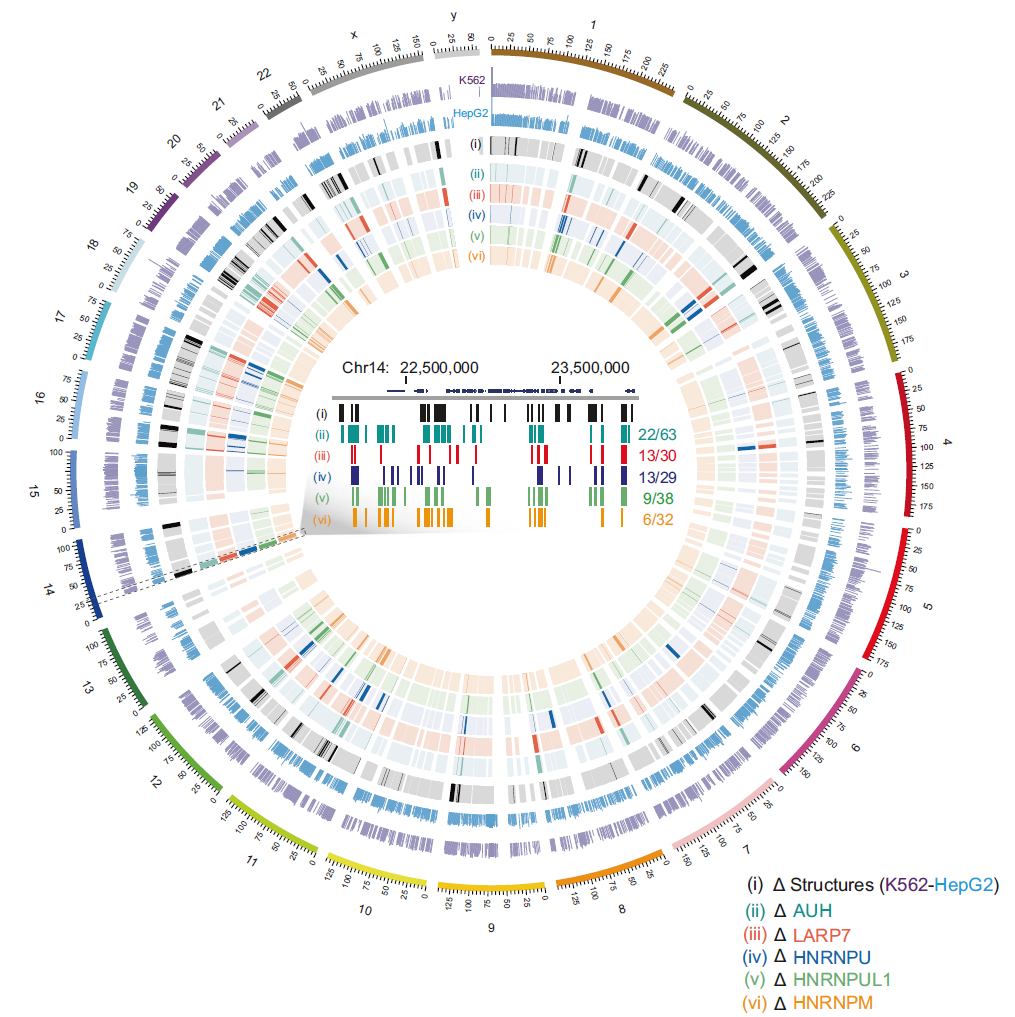
\includegraphics[width=\textwidth]{./figures/relation1.png}
        \label{fig:relation1}
      \end{figure}
    \end{column}
    \begin{column}{0.5\textwidth}
      \begin{figure}[H]
        \raggedleft
        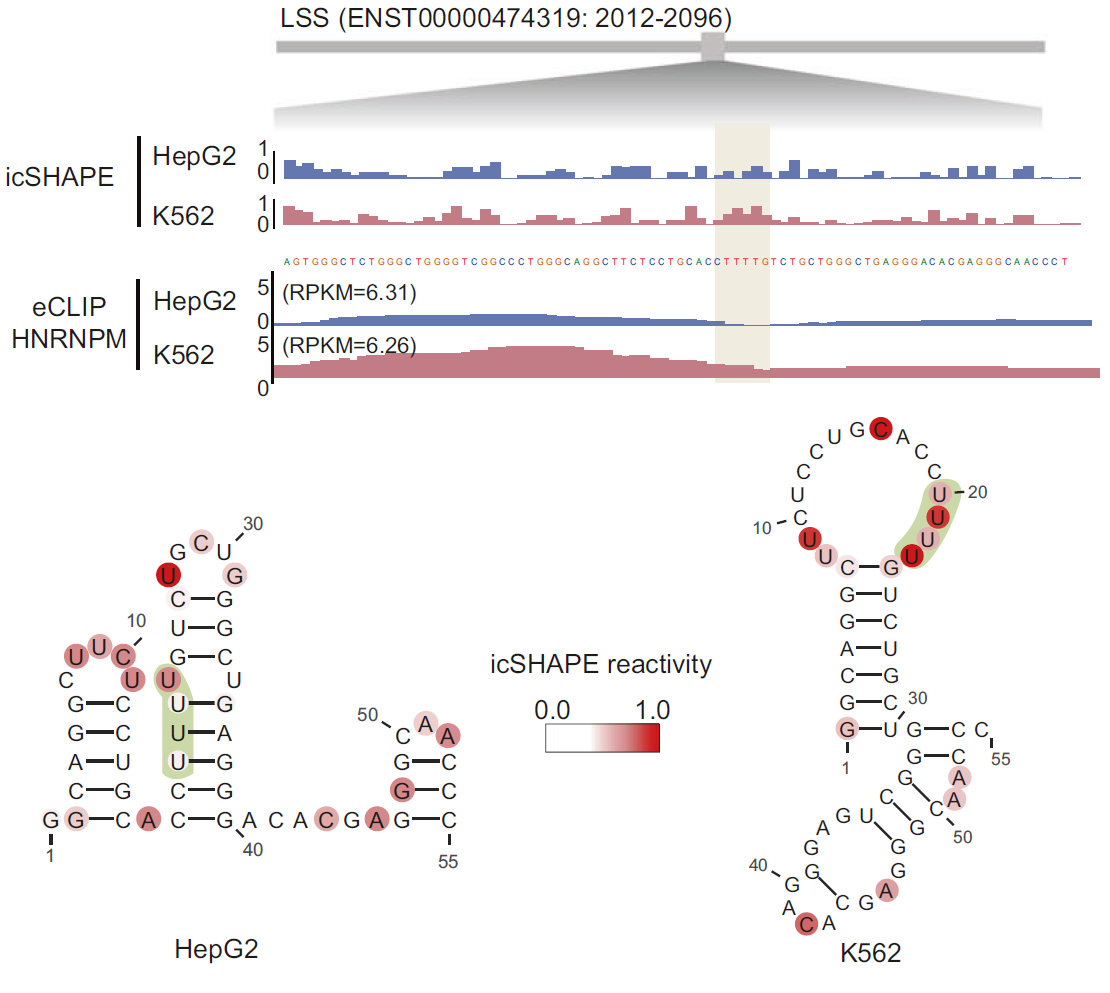
\includegraphics[width=\textwidth]{./figures/snapshot.png}
        \label{fig:snapshot}
      \end{figure}
    \end{column}
  \end{columns}
  \begin{block}{Conclusion}
  dynamic RBP binding sites are associated with the RNA structurally variable sites between the two cell types
  \end{block}
\end{frame}

\section{Performance}
\begin{frame}
  \frametitle{AUC}
    \begin{columns}[T]
    \begin{column}{0.5\textwidth}  
  \begin{figure}[H]
    \raggedright
    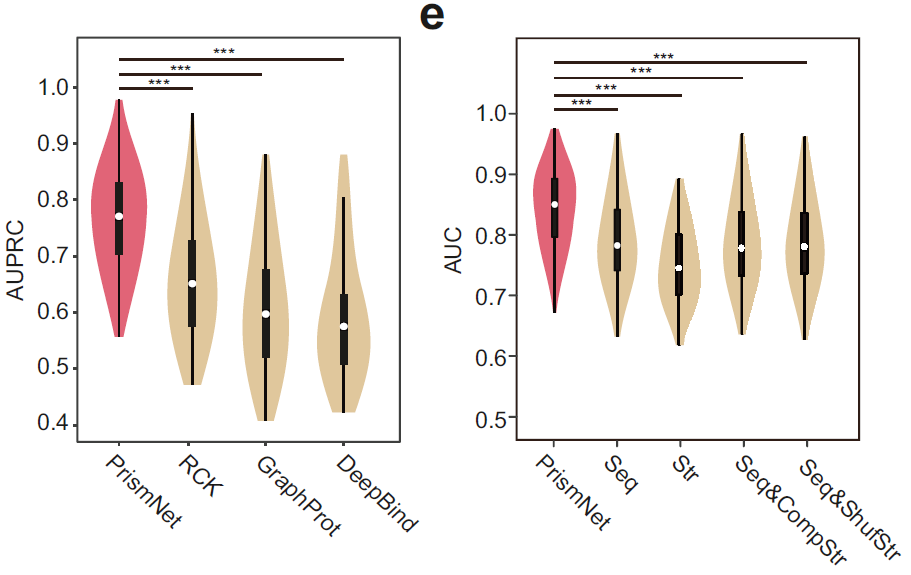
\includegraphics[width=\textwidth]{./figures/auc_models.png}
    \caption{Better than other methods}
    \label{fig:metods}
      \end{figure}
    \end{column}
    \begin{column}{0.5\textwidth}
  \begin{figure}[H]
    \raggedleft
    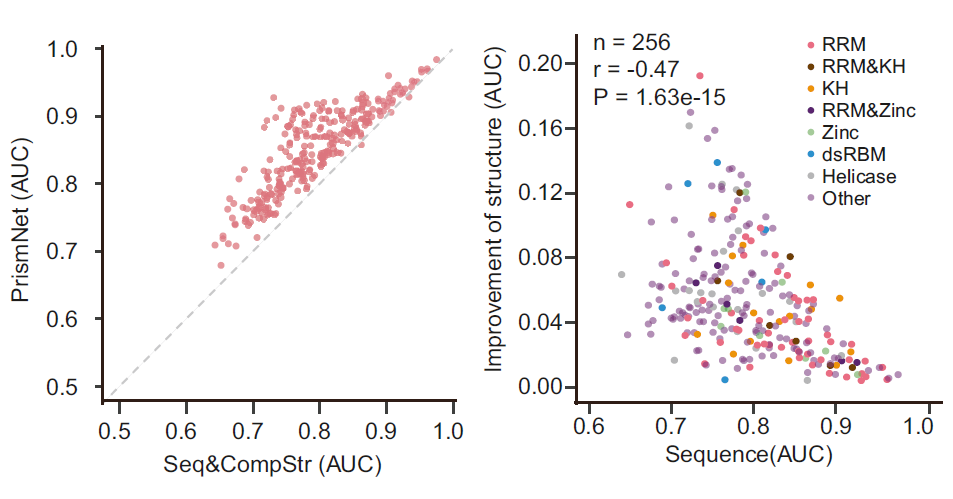
\includegraphics[width=\textwidth]{./figures/auc_input.png}
    \caption{Better than one input}
    \label{fig:inputs}
  \end{figure}
  \end{column}
  \end{columns}
\end{frame}

\begin{frame}
  \frametitle{Predicted Output Values}
  \begin{figure}[H]
    \center
    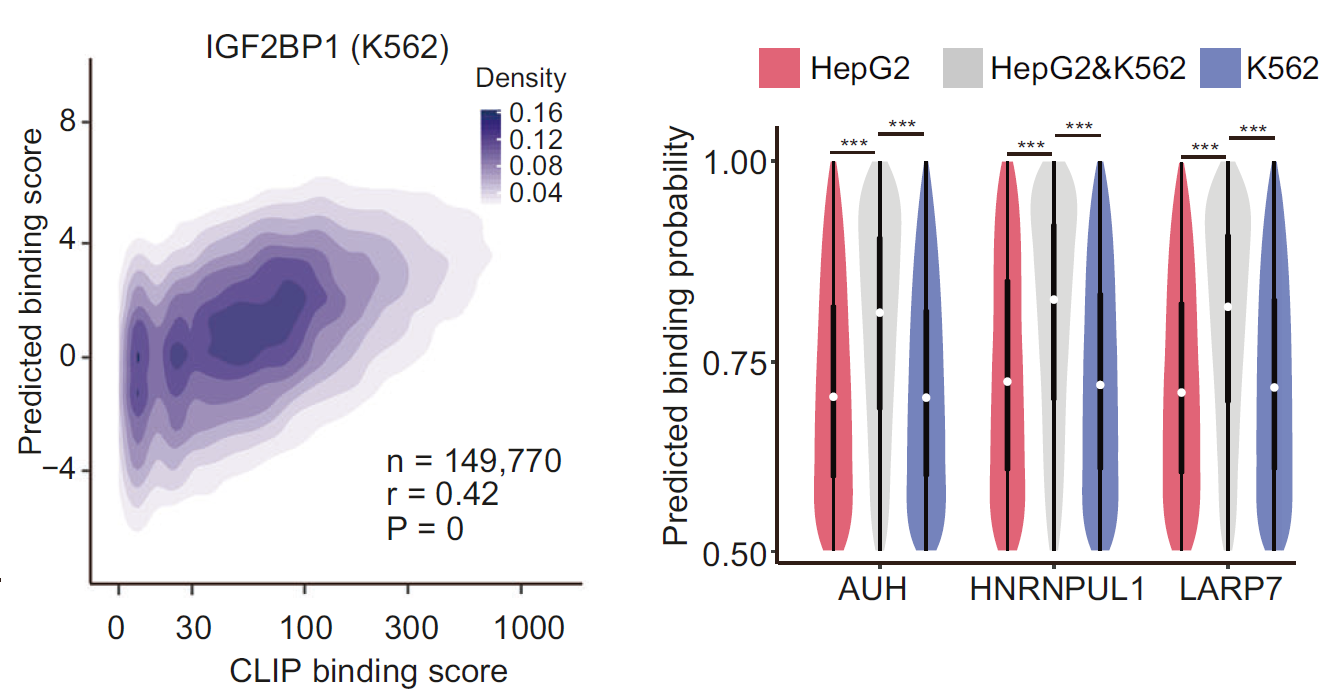
\includegraphics[width=0.85\textwidth]{./figures/predict_out.png}
    %\caption{REctified Linear Unit}
    \label{fig:predict_out}
  \end{figure}
  \begin{block}{Conclusion}
  cell type-specific binding sites generally had lower predicted binding scores compared to common binding sites
  \end{block}
\end{frame}

\begin{frame}
  \frametitle{Experimental Validation}
  \begin{figure}[H]
    \center
    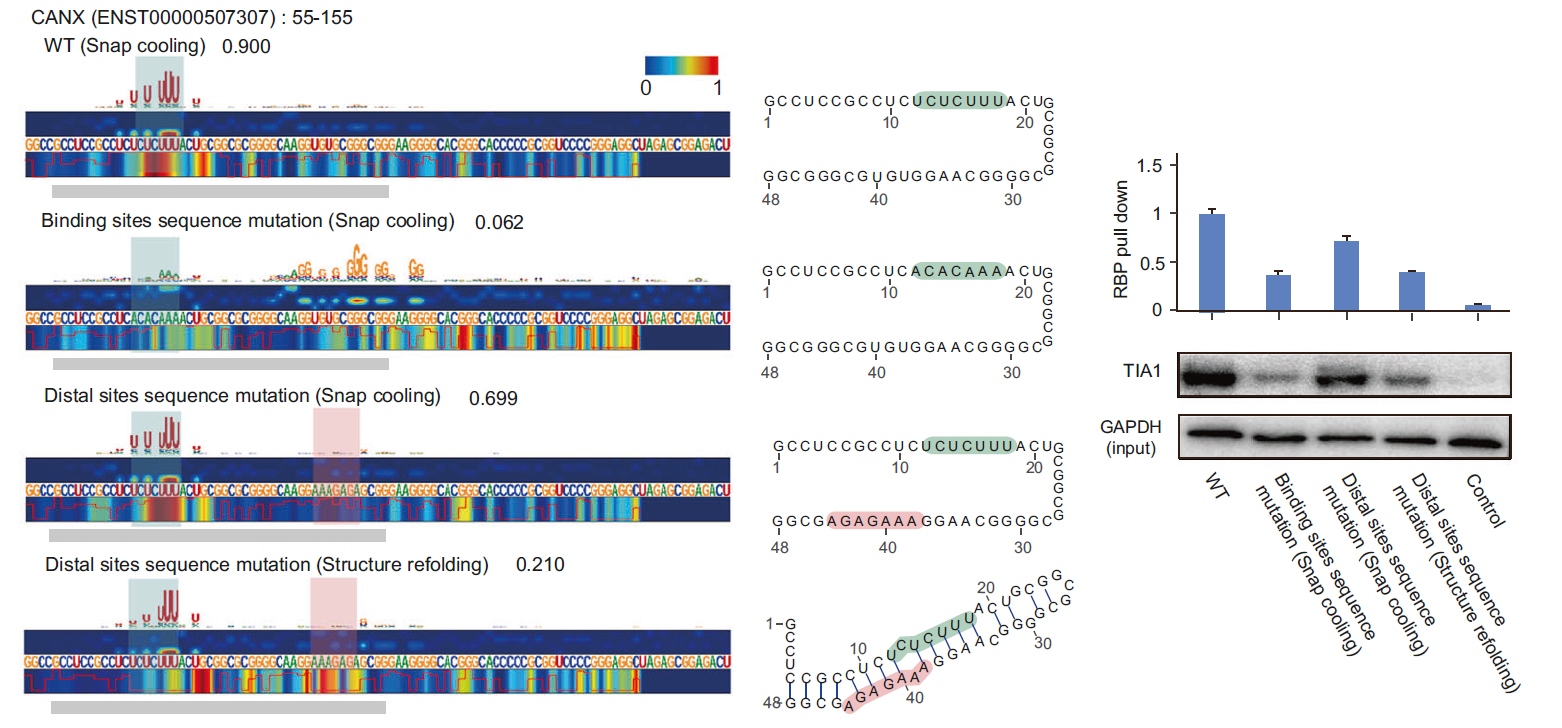
\includegraphics[width=0.85\textwidth]{./figures/validation.png}
    \caption{validated the structural preferences
of TIA1 for single-stranded conformation}
    \label{fig:validation}
  \end{figure}
  \begin{block}{Conclusion}
  PrismNet accurately predicted the structural preference of RBPs
  \end{block}
\end{frame}

\section{Applications}
\begin{frame}
  \frametitle{Predicting SV and RNA binding}
  \begin{figure}[H]
    \center
    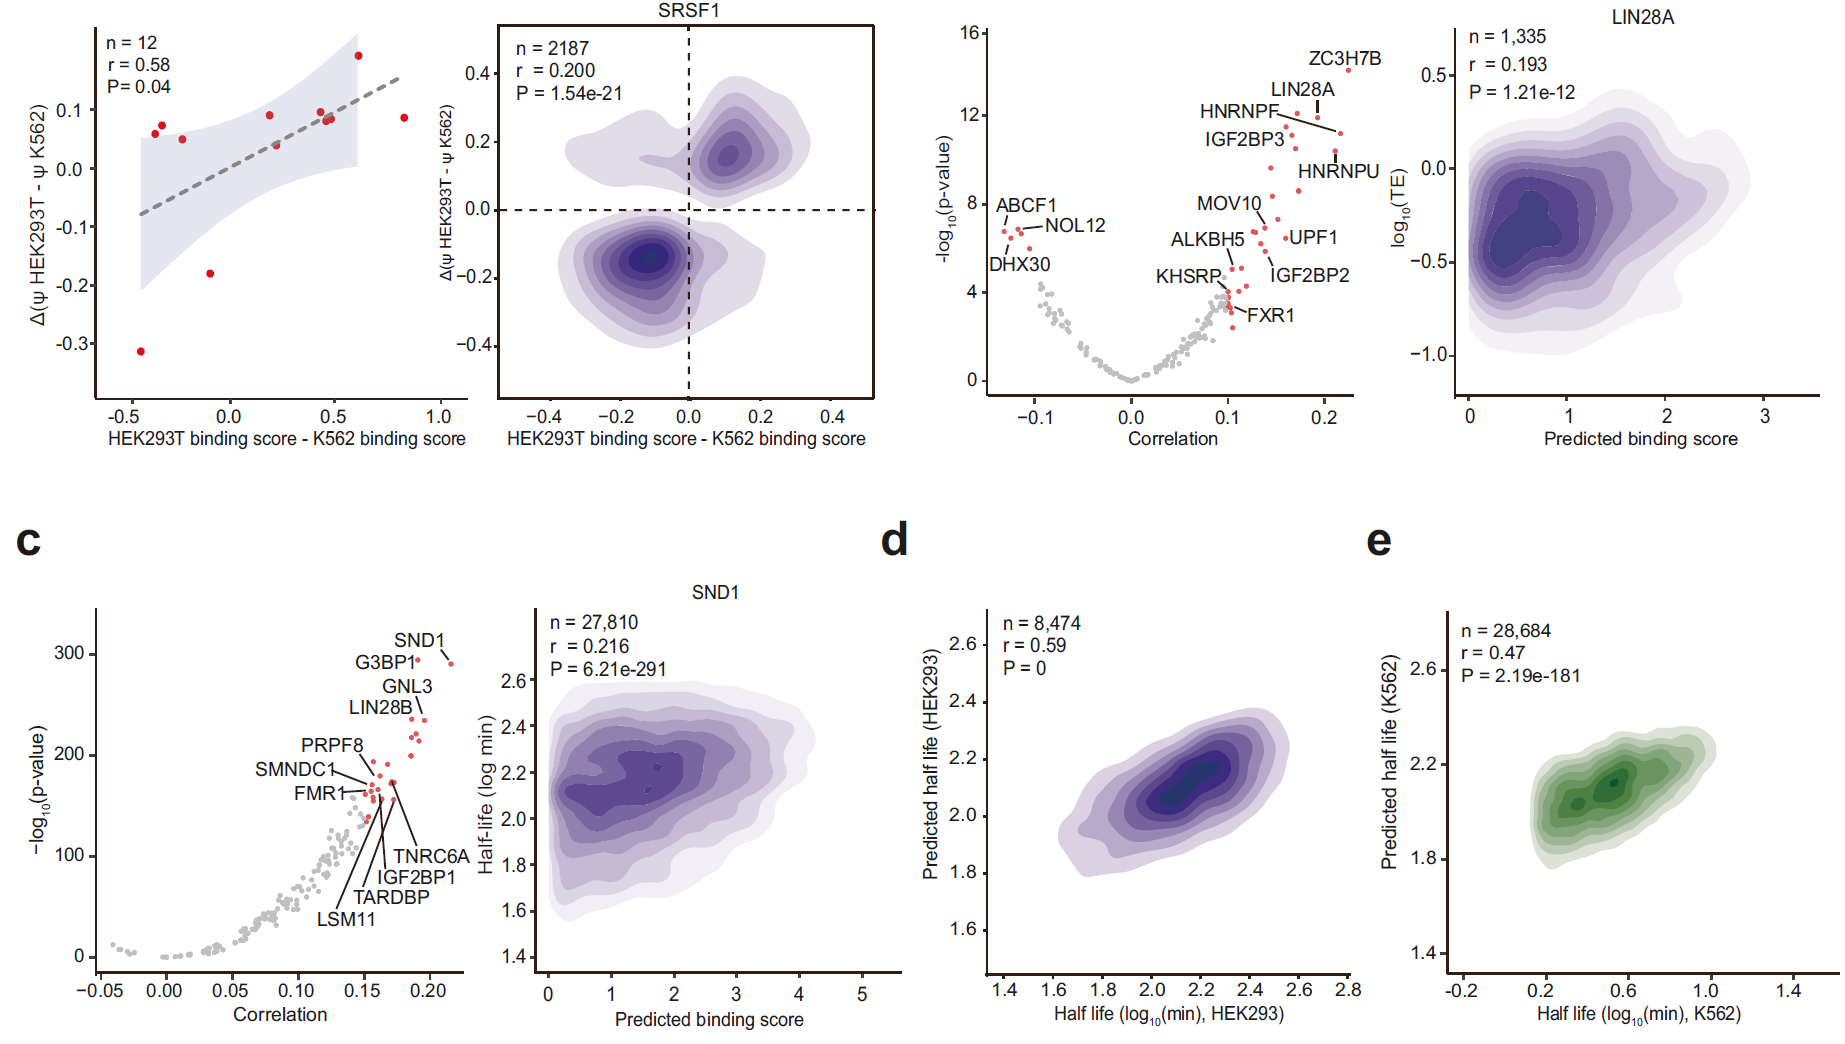
\includegraphics[width=0.85\textwidth]{./figures/predict.png}
    %\caption{REctified Linear Unit}
    \label{fig:predict}
  \end{figure}
  \begin{block}{Conclusion}
  PrismNet predictions reveal putative regulators in posttranscriptional
regulation events
  \end{block}
\end{frame}

\begin{frame}
  \frametitle{Finding Motifs}
  \begin{figure}[H]
    \center
    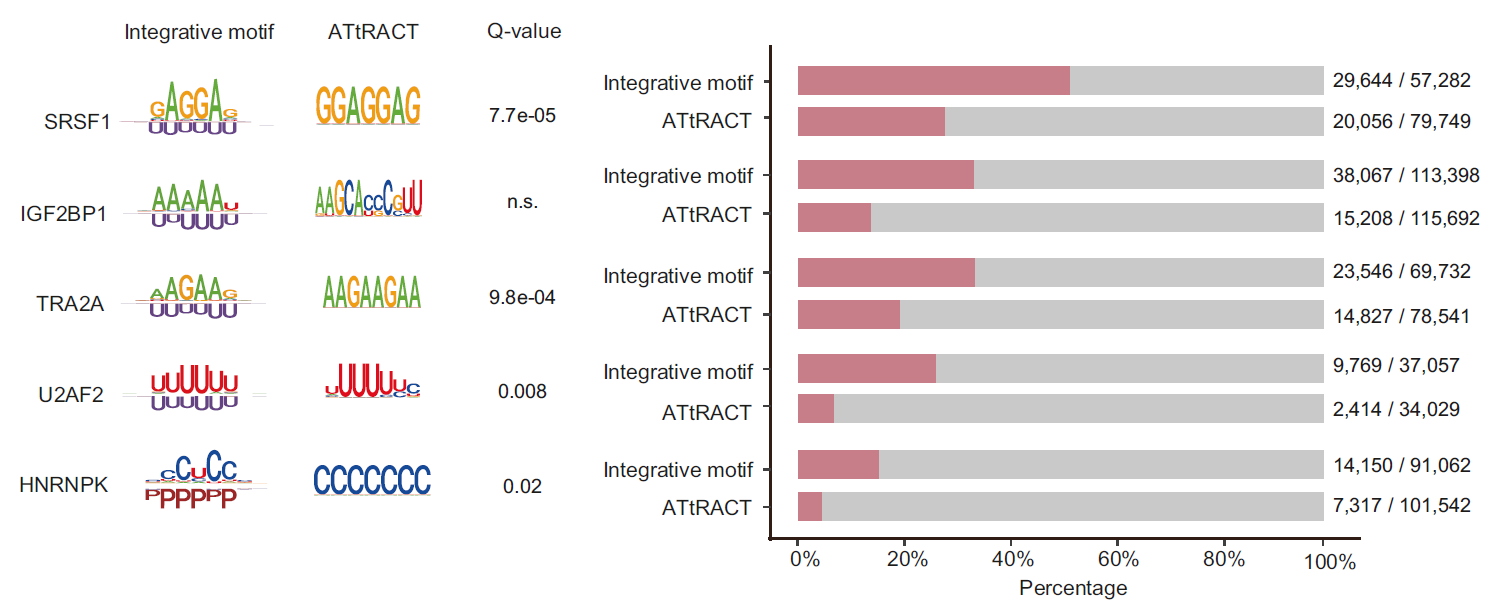
\includegraphics[width=\textwidth]{./figures/motif1.png}
    \caption{More True Positive}
    \label{fig:motif1}
  \end{figure}
\end{frame}

\begin{frame}
  \frametitle{Finding Motifs}
  \begin{figure}[H]
    \center
    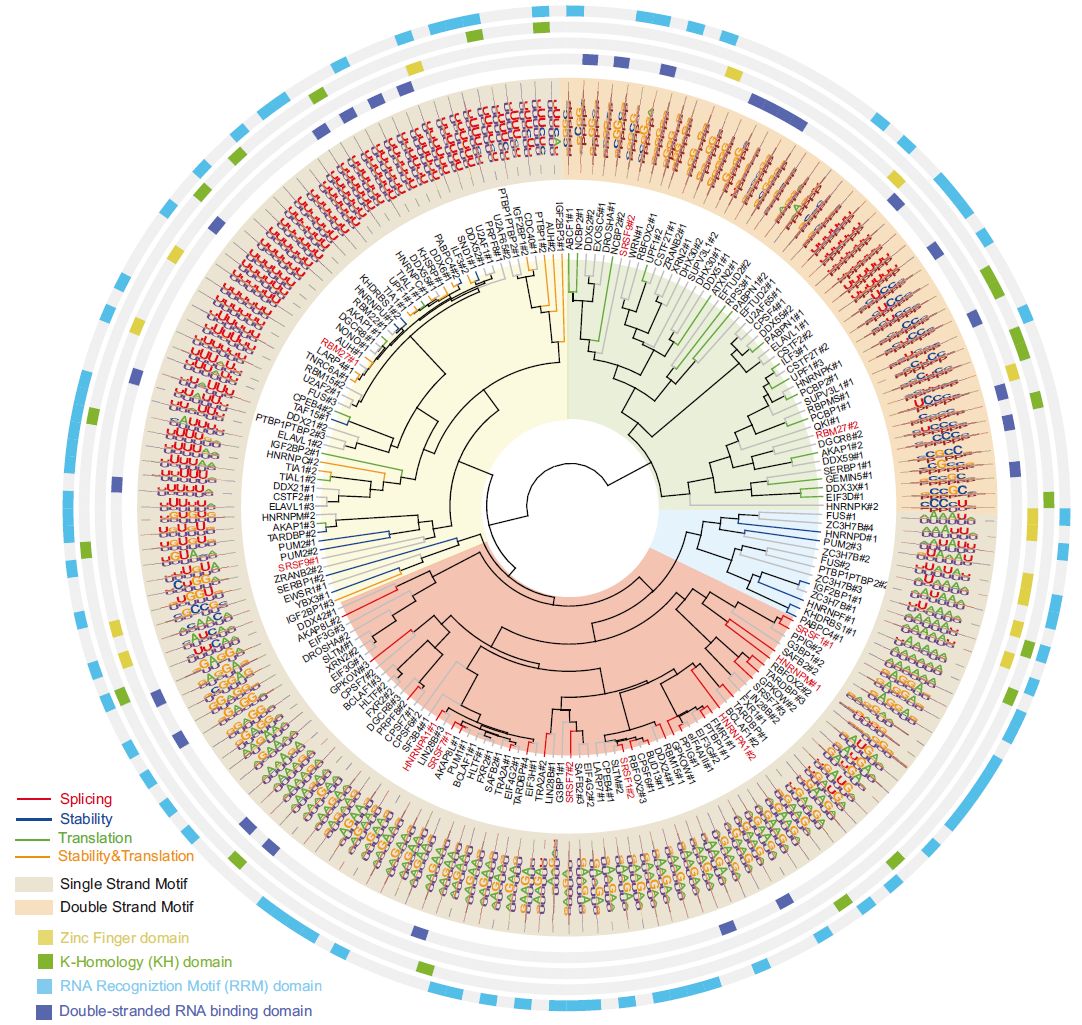
\includegraphics[width=0.7\textwidth]{./figures/motif2.png}
    \caption{Clustering Well}
    \label{fig:motif2}
  \end{figure}
\end{frame}

\begin{frame}
  \frametitle{HARs}
  \begin{figure}[H]
    \center
    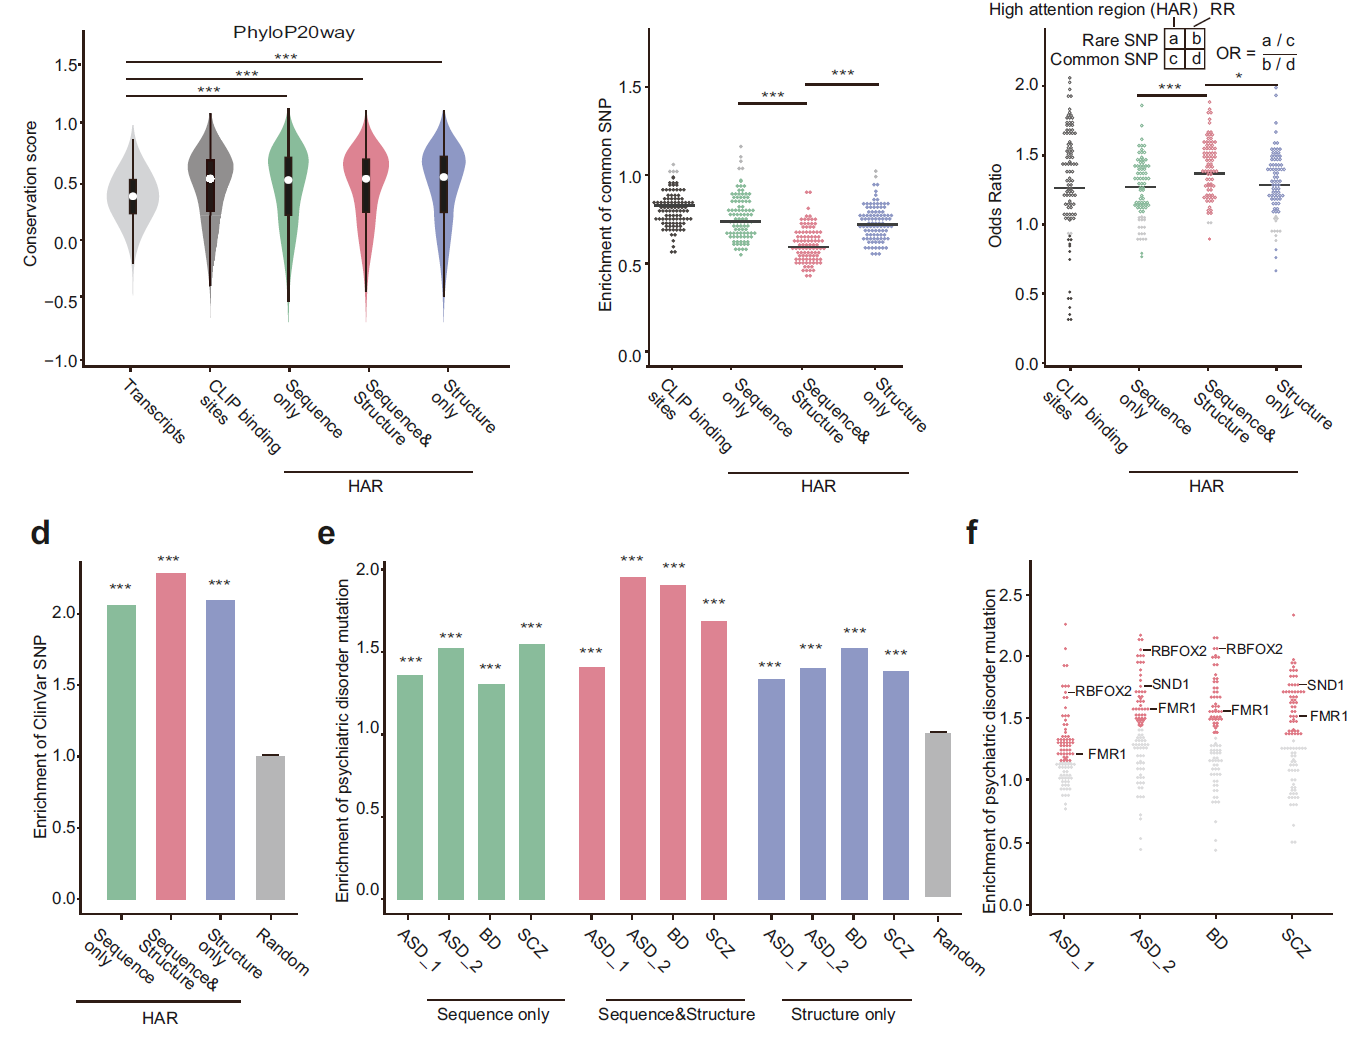
\includegraphics[width=0.7\textwidth]{./figures/har.png}
    %\caption{Clustering Well}
    \label{fig:har}
  \end{figure}
    \begin{block}{Conclusion}
    HARs(high attention regions (HARs), which are predicted to be the
exact locations of RBP binding nucleotides) are more evolutionarily conserved
  \end{block}
\end{frame}

\begin{frame}
  \frametitle{RiboSNitches}
  \begin{figure}[H]
    \center
    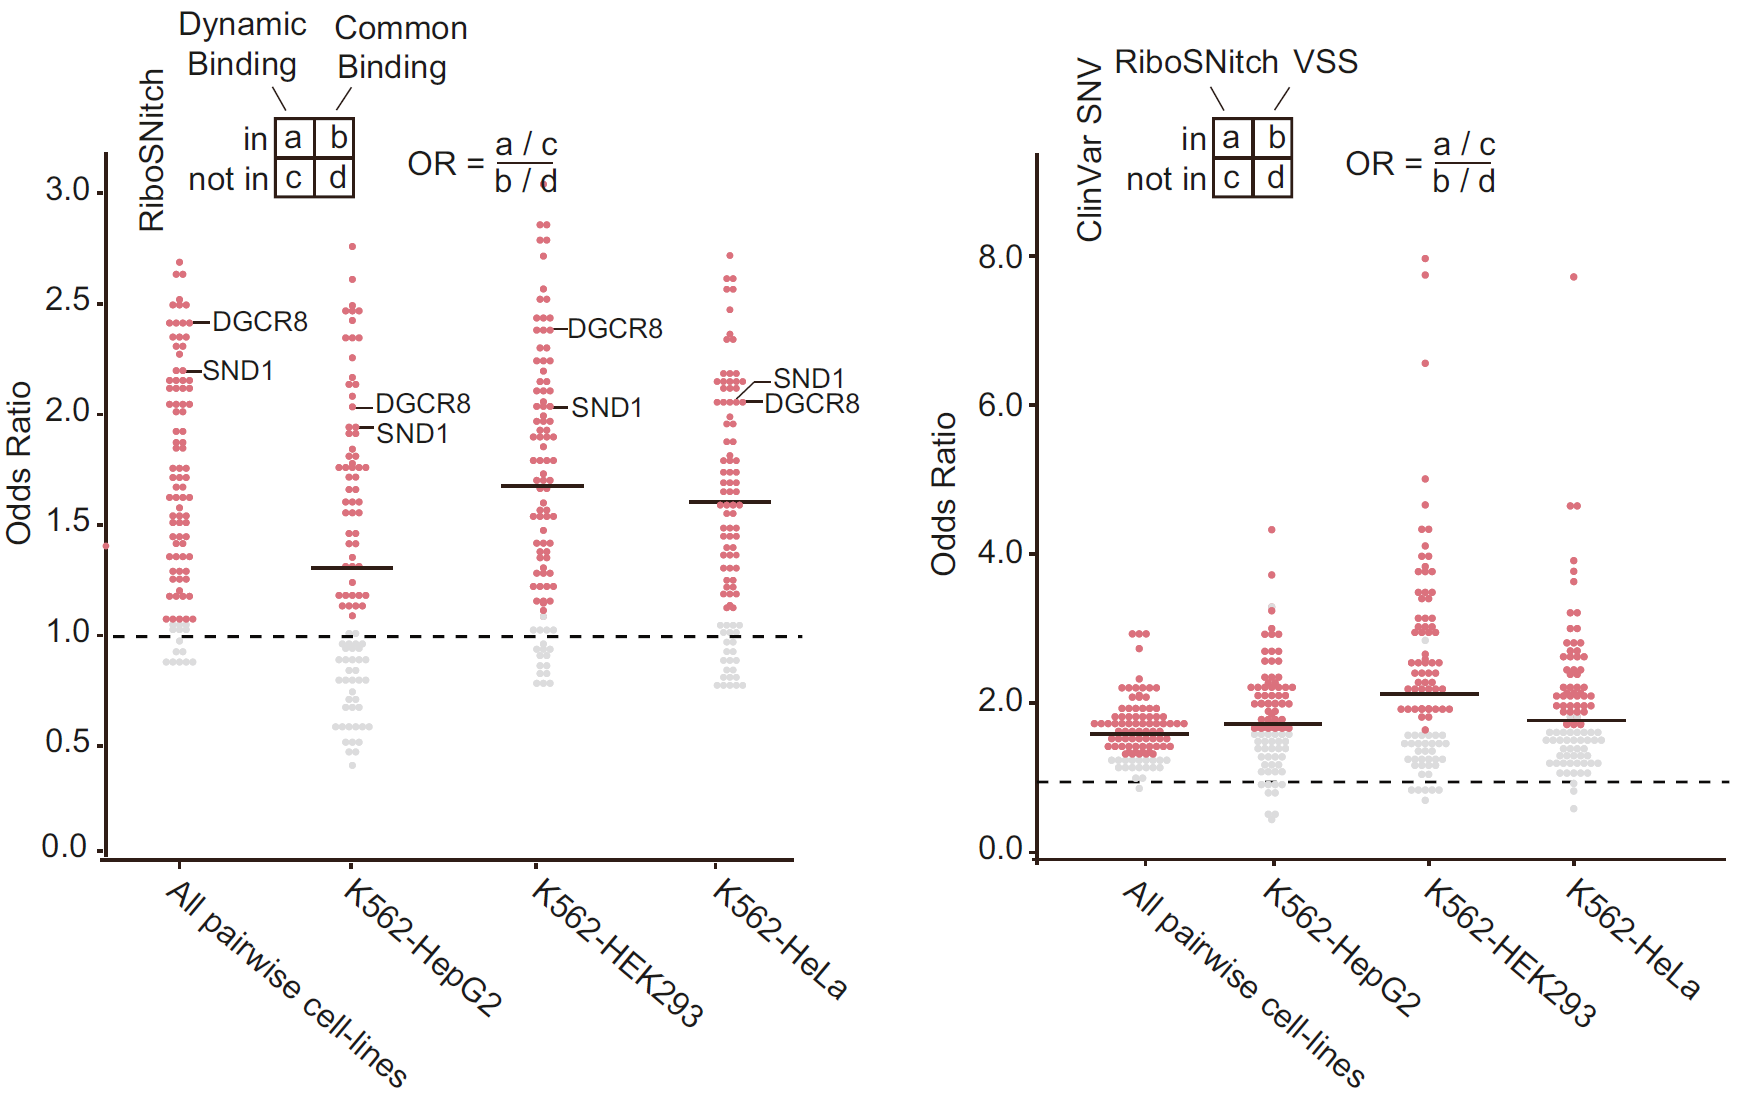
\includegraphics[width=0.8\textwidth]{./figures/ribosnitch1.png}
    %\caption{Clustering Well}
    \label{fig:rn1}
  \end{figure}
    \begin{block}{Conclusion}
    for most RBPs, their dynamic binding sites are enriched with riboSNitches( The SNVs that affected RSS)
  \end{block}
\end{frame}

\begin{frame}
  \frametitle{RiboSNitches-PNPO}
  \begin{figure}[H]
    %\center
    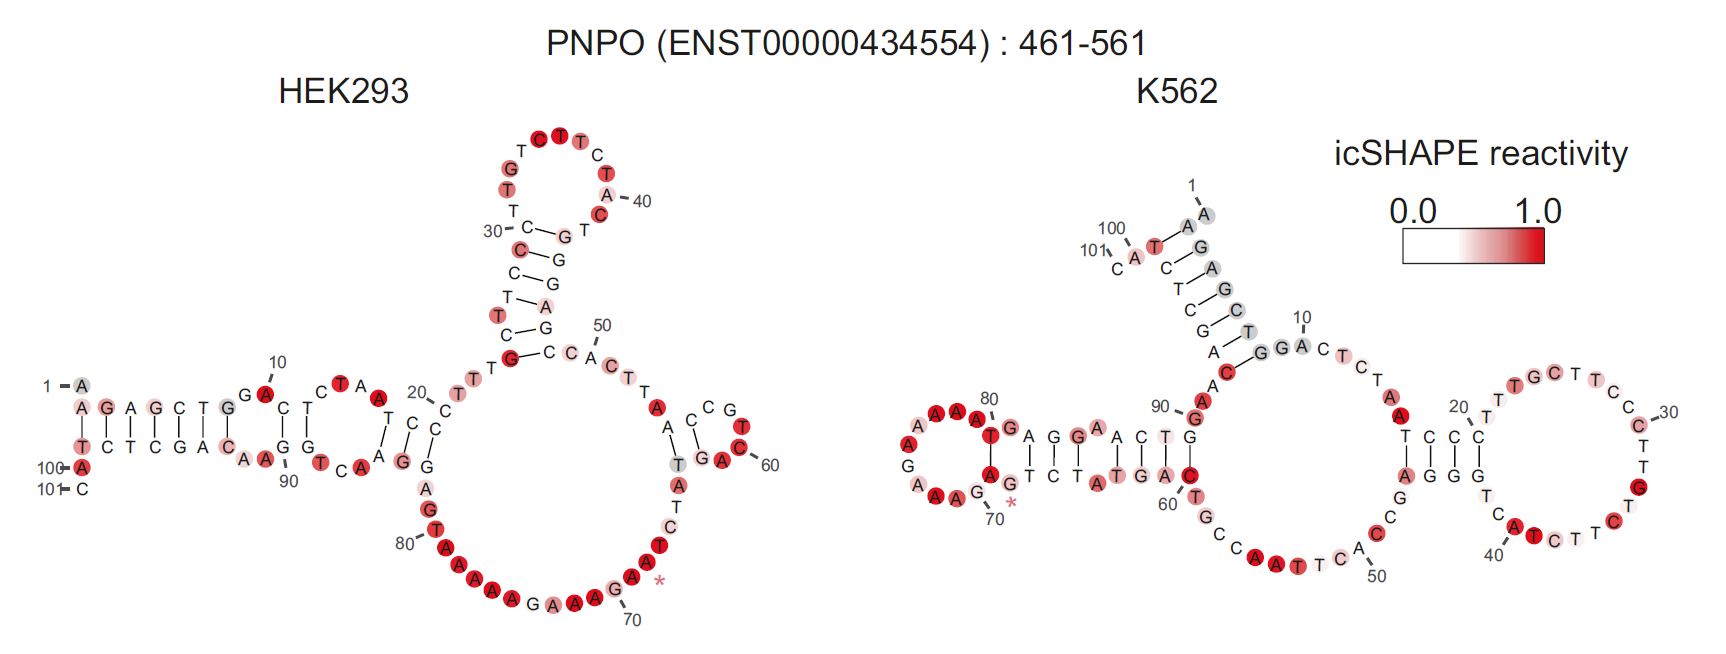
\includegraphics[width=0.5\textwidth]{./figures/PNPO1.png}
    %\caption{Clustering Well}
    \label{fig:rn1}
  \end{figure}
  \begin{figure}[H]
    %\center
  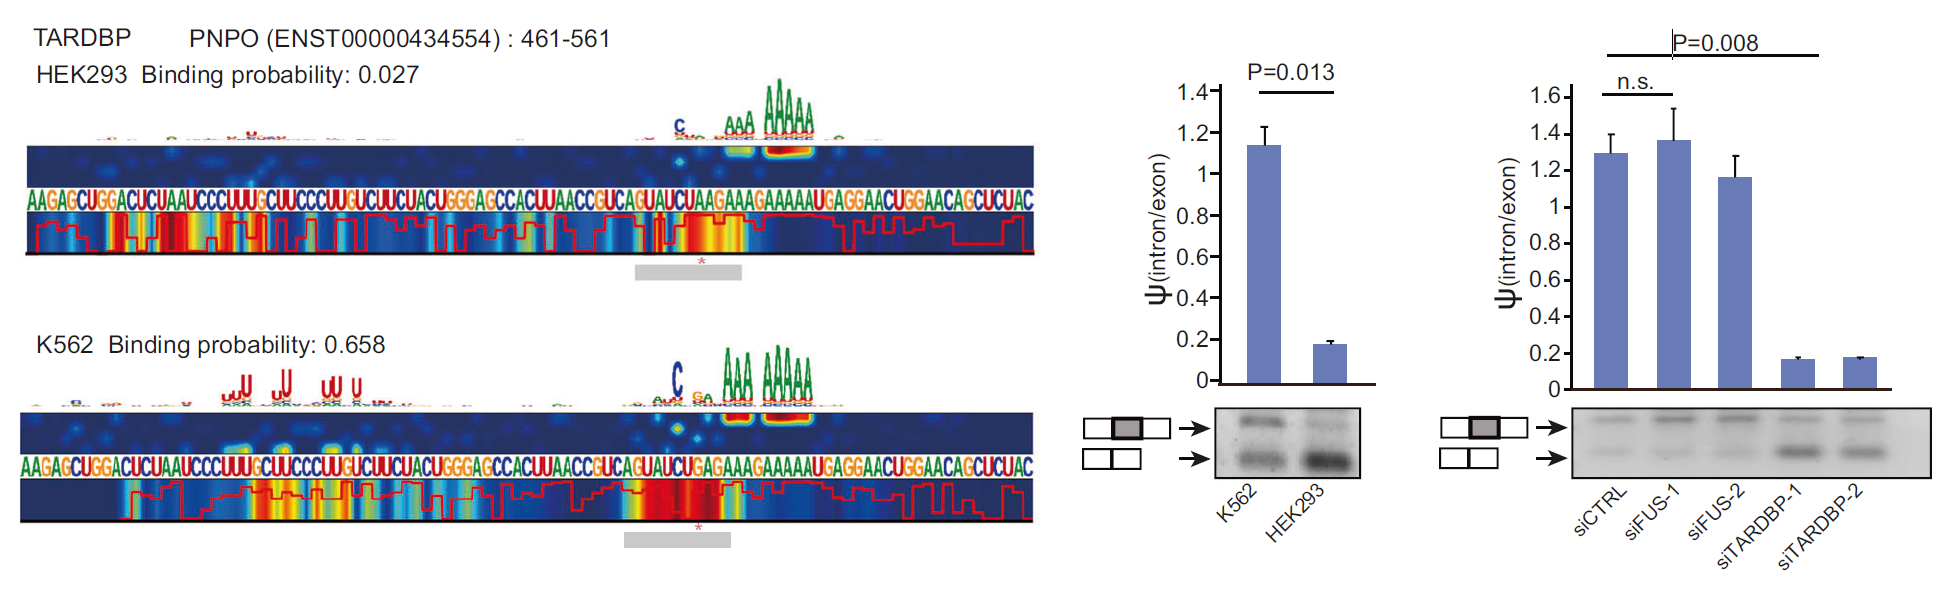
\includegraphics[width=0.8\textwidth]{./figures/pnpo2.png}
    %\caption{Clustering Well}
  \label{fig:rn1}
  \end{figure}
    \begin{block}{Term}
    The exon-inclusion ratio: how often the exon occurs in all the isoforms of the gene that contains the exon
  \end{block}
\end{frame}

\begin{frame}
  \frametitle{Acknowledgement}
  \centerline{\Large Thanks for Your Listening!}
\end{frame}

\end{document}
